% Physical Review E -- standalone Supplemental Material working draft.
% Scientific claim boundary checked against repository artifacts on 2026-07-11.
% Supplemental Material source (single author, revised 2026-07-30).
\documentclass[aps,pre,reprint,amsmath,amssymb,longbibliography,floatfix]{revtex4-2}

\usepackage{cmap}
\usepackage[T1]{fontenc}
\usepackage{lmodern}
\usepackage{graphicx}
\usepackage{bm}
\usepackage{booktabs}
\usepackage{hyperref}
\hypersetup{
  hidelinks,
  pdftitle={Supplemental Material: Spectral diagnostics and local fixed-budget sensitivity of critical points in finite encounter-reaction models},
  pdfauthor={Xiaoxiao Zhouyi},
  pdfsubject={Detailed derivations and finite-model audits for encounter-reaction time modality},
  pdfkeywords={encounter reaction, reaction-time density, multimodality, Doi model, Green operator, modality fold}
}
\usepackage{placeins}

\graphicspath{{../artifacts/figures/}{./figures/}{./}}
\renewcommand{\topfraction}{0.92}
\renewcommand{\textfraction}{0.05}
\renewcommand{\floatpagefraction}{0.82}

\newcommand{\Dr}{D_{\mathrm r}}
\newcommand{\Dc}{D_{\mathrm c}}
\newcommand{\keff}{k_{\mathrm{eff}}}
\newcommand{\Da}{\mathrm{Da}}
\newcommand{\dd}{\mathrm d}
\newcommand{\e}{\mathrm e}
\newcommand{\Tgen}{\mathcal T}
\newcommand{\Lfree}{\mathcal L_0}
\newcommand{\Rfree}{\mathcal R_0}
\newcommand{\Gres}{\mathcal G}

% This file compiles without the main-paper .aux.  Supplemental counters carry
% an S prefix; references are resolved solely from this file's own auxiliary
% data and therefore do not depend on labels emitted by the main article.
\renewcommand{\thesection}{S\arabic{section}}
\renewcommand{\thesubsection}{S\arabic{section}.\arabic{subsection}}
\renewcommand{\thesubsubsection}{S\arabic{section}.\arabic{subsection}.\arabic{subsubsection}}
\renewcommand{\theequation}{S\arabic{equation}}
\renewcommand{\thefigure}{S\arabic{figure}}
\renewcommand{\thetable}{S\Roman{table}}
\makeatletter
\renewcommand{\p@subsection}{}
\renewcommand{\p@subsubsection}{}
\makeatother

\begin{document}

\title{Supplemental Material for: Spectral diagnostics and local fixed-budget sensitivity of critical points in finite encounter-reaction models}

\author{Xiaoxiao Zhouyi}
\email{xiaoxiao.zhouyi@bristol.ac.uk}
\affiliation{School of Engineering Mathematics and Technology, University of Bristol,
Bristol BS8 1TW, United Kingdom}

\date{July 30, 2026}

\begin{abstract}
This Supplemental Material is a standalone detailed record for the associated
article. It gives the full coordinate and reaction-model qualifications,
finite-support Green and spectral audits, generalized-inverse-Gaussian
screening construction, finite-state discovery and clock controls, complete
two-dimensional discretization and endpoint families, capacity calibrations,
multichannel screening calculations, normal-form derivations, provenance
boundary, and limitations. The main article retains only the Green--Woodbury
reduction, the necessary spectral gate, fixed-budget sensitivity, the finite
CTMC fold, and the M2D-F finite-generator fold certificate. All results here
remain finite-model or screening statements unless an exact identity is
explicitly identified; no continuum modality theorem is asserted.
\end{abstract}

\maketitle

\section{Scope and detailed evidence map}
\label{sec:introduction}

This file is the technical companion to the focused main article, not a second
statement of its narrative. It retains the full model qualifications,
derivations, secondary finite-grid families, screening calculations,
provenance boundary, and limitations needed to audit the evidence. The present
work is a direct extension of that encounter and heterogeneous-transmission
program; it does not claim a new Green, multi-target, fold-criterion, or
fixed-total-reactivity theory. The finite evidence uses separately declared
M2D-E, M2D-F, M2D-C, and M2D-T families. No common continuation relation
between M2D-E and M2D-F is asserted.

Three evidence levels remain separate throughout: exact identities under
stated hypotheses, certificates for declared finite generators, and numerical
screening or continuum-consistency evidence. In particular, the finite-grid
folds and endpoint audits do not establish a continuum modality theorem.

Table~\ref{tab:evidence} fixes the evidence level and corresponding claim
boundary for every analytical and numerical layer used below.

\begin{table*}[!t]
\caption{\label{tab:evidence}
Statement/evidence boundary used in this manuscript.}
\begin{ruledtabular}
\begin{tabular}{p{0.25\textwidth}p{0.27\textwidth}p{0.39\textwidth}}
Statement & Evidence level & Boundary\\
\hline
Coordinate decoupling, mass balance, Woodbury reduction, fixed-shape fold,
generic normal form
& Exact identities under stated algebraic or operator hypotheses
& Inverse-free volume-reaction identity; no continuum meromorphic continuation,
bounded-coordinate independence, or unqualified Robin trace claim\\
Finite reversible spectral diagnostic
& Classical generalized-Descartes corollary plus spectral reconstructions of
the 961-state encounter and 2025-state M2D-T primary generators
& Necessary sign-variation bound only; not sufficient, not a channel-rank
bound, and not applied to complex-spectrum, Jordan, or continuum laws; this is
a loose consistency/falsification gate, not independent root discovery\\
Fixed-budget modality susceptibility
& Exact finite Fr\'echet--Duhamel identity, closed-form projected optimum, 256
independent directions, and 20,000 random feasible controls
& Infinitesimal interior-rate design only; no finite-amplitude, binary-mask,
moving-support, or continuum optimum is claimed\\
Finite CTMC physical fold
& Finite-matrix derivative identities evaluated numerically, plus a root solve and independent
continuation
& One finite model; minority splitting probability
\(8.95\times10^{-6}\)\\
M2D-F matched-budget folds
& Three nondegenerate finite-generator folds and a budget-measure control
& Separate finite-model mechanism certificates; fold coordinates span
\(0.262\) and move under product-control-volume weighting; no common
continuation with M2D-E or continuum critical value is claimed\\
M2D-E equal-budget endpoint amplification
& A five-grid resolution, tail, morphology, and 101-cutoff audit
& Four finer patterned endpoints are resolved-bimodal and the coarse endpoint
is a shoulder; the cutoff interval is post-hoc and sample-derived, not a
detector/noise-robustness result; no M2D-E fold is claimed\\
2D catalytic-coordinate sensitivity
& One-factor midpoint/weighted comparison on three principal grids
& Labels agree but masks and densities change; the physical sink models are not equivalent\\
Bounded 2D three-channel trimodality
& Five detected sign-changing derivative roots of alternating type (hence at
least five positive-time roots) and ordered channel attribution on four finite
grids;
three classifier-resolved trimodal cases and one three-maximum shoulder
& Patch radii are below \(h_x\), reactive-state counts are nonmonotone, and
there is no interval-exhaustive root certificate, cell-averaged continuum
trimodal region, or phase boundary\\
2D and 3D capacity laws
& Translation-invariant relative-coordinate mean-time calculations
& Not centre-patterned density or modality calculations\\
Multidimensional multi-channel GIG construction
& Exact design algebra plus floating-point derivative-root isolation in 12
declared screening cases
& Not a bounded Doi three- or four-mode theorem\\
GIG encounter channels
& Exact GIG algebra, approximate mapping from free encounter geometry
& No uniform confined-channel remainder
\end{tabular}
\end{ruledtabular}
\end{table*}

The spatial-channel schematic and generic fold geometry appear as Fig.~1 of
the main article. The supplemental record therefore begins directly with the
model qualifications and derivations rather than duplicating that figure.

\section{Finite-radius patterned encounter model}
\label{sec:model}

\subsection{Joint dynamics and reaction channels}
\label{sec:joint}

Let \(X_i(t)\in\Omega\subset\mathbb R^d\) denote two independent particles
before reaction,
\begin{equation}
\dd X_i=b_i(X_i)\,\dd t+\sqrt{2D_i}\,\dd W_i,
\qquad D_i>0,\quad i=1,2,
\label{eq:sde}
\end{equation}
with independent Brownian motions. We use reflecting outer boundaries unless
stated otherwise. The unreacted joint density \(p(x_1,x_2,t)\) satisfies
\begin{equation}
\partial_t p=\Lfree p-K(x_1,x_2)p,
\label{eq:joint-fp}
\end{equation}
\begin{equation}
\Lfree p=-\nabla_{x_1}\!\cdot(b_1p)
         -\nabla_{x_2}\!\cdot(b_2p)
         +D_1\Delta_{x_1}p+D_2\Delta_{x_2}p,
\label{eq:free-generator}
\end{equation}
with no-flux currents \(J_i=b_ip-D_i\nabla_{x_i}p\).

The finite contact radius is \(a>0\). A physical catalyst must also declare
which affine location of the pair it reads:
\begin{equation}
C_\eta(x_1,x_2)=\eta x_1+(1-\eta)x_2,
\qquad 0\leq\eta\leq1.
\label{eq:catalytic-coordinate}
\end{equation}
Catalytic patch \(C_j\) is specified in this \(C_\eta\)-space, with intrinsic
Doi rate \(\kappa_j(C_\eta)\geq0\). The channel-resolved killing fields are
\begin{align}
K_{a,j}^{(\eta)}(x_1,x_2)
&=\kappa_j(C_\eta)\mathbf 1_{C_j}(C_\eta)
  \mathbf 1_{\{|x_1-x_2|<a\}},\notag\\
K_a^{(\eta)}&=\sum_{j=1}^m K_{a,j}^{(\eta)}.
\label{eq:doi-killing}
\end{align}
The survival probability and reaction-channel densities are
\begin{align}
S(t)&=\int_{\Omega^2}p(x_1,x_2,t)\,\dd x_1\,\dd x_2,\\
f_j(t)&=\int_{\Omega^2}K_{a,j}^{(\eta)}(x_1,x_2)
p(x_1,x_2,t)\,\dd x_1\,\dd x_2,
\label{eq:channel-flux}
\end{align}
Reflecting outer boundaries give the exact mass balance
\begin{equation}
-S'(t)=f(t)=\sum_{j=1}^m f_j(t).
\label{eq:mass-balance}
\end{equation}
The splitting probability into channel \(j\) is
\(\pi_j=\int_0^\infty f_j(t)\,\dd t\); when reaction is certain,
\(\sum_j\pi_j=1\), and \(g_j=f_j/\pi_j\) is the conditional channel-time
density.

\subsection{Relative, diffusion-decoupling, and catalytic coordinates}
\label{sec:coordinates}

Set
\begin{equation}
\Dr=D_1+D_2,\qquad
\Dc=\frac{D_1D_2}{D_1+D_2},
\label{eq:relative-diff}
\end{equation}
and define
\begin{equation}
r=X_1-X_2,\qquad
R=\frac{D_2X_1+D_1X_2}{D_1+D_2}.
\label{eq:coordinates}
\end{equation}
The catalytic coordinate in Eq.~\eqref{eq:catalytic-coordinate} is related to
the diffusion-decoupling coordinate by
\begin{equation}
C_\eta=R+\left(\eta-\frac{D_2}{\Dr}\right)r.
\label{eq:ceta-relation}
\end{equation}
Hence \(C_{D_2/\Dr}=R\). The bounded two-dimensional calculations below use
the physical midpoint convention
\begin{align}
C_{1/2}&=\frac{X_1+X_2}{2}
=R+\frac{D_1-D_2}{2\Dr}r,\notag\\
|C_{1/2}-R|&\leq\frac{|D_1-D_2|}{2\Dr}a,
\qquad |r|<a.
\label{eq:midpoint-shift}
\end{align}
The inverse map is
\begin{equation}
x_1=R+\frac{D_1}{\Dr}r,\qquad
x_2=R-\frac{D_2}{\Dr}r,
\label{eq:coordinate-inverse}
\end{equation}
and the absolute Jacobian is one. Direct substitution gives the exact
cancellation
\begin{equation}
D_1\Delta_{x_1}+D_2\Delta_{x_2}
=\Dr\Delta_r+\Dc\Delta_R.
\label{eq:diffusion-decoupling}
\end{equation}
Thus
\begin{align}
\partial_tq={}&-\nabla_r\!\cdot(uq)-\nabla_R\!\cdot(v_{\mathrm c}q)
 +\Dr\Delta_rq+\Dc\Delta_Rq\notag\\
&-K_a^{(\eta)}(x_1(R,r),x_2(R,r))q,
\label{eq:transformed-fp}
\end{align}
where
\begin{equation}
u=b_1(x_1)-b_2(x_2),\qquad
v_{\mathrm c}=\frac{D_2b_1(x_1)+D_1b_2(x_2)}{\Dr}.
\label{eq:transformed-drifts}
\end{equation}
For constant drifts in free space, relative and centre noises are independent.
This statement must not be transferred unqualified to bounded domains: the
transformed domain
\begin{equation}
\mathcal D=\left\{(R,r):
R+\frac{D_1}{\Dr}r\in\Omega,\quad
R-\frac{D_2}{\Dr}r\in\Omega\right\}
\label{eq:transformed-domain}
\end{equation}
has coupled boundaries. Nonconstant drifts can also couple \(r\) and \(R\).
The weighted coordinate in Eq.~\eqref{eq:coordinates} is selected by diffusion,
not imposed as the physical catalyst location. In \((r,C_\eta)\) coordinates,
the centre diffusivity is
\(D_\eta=D_1\eta^2+D_2(1-\eta)^2\) and the mixed second-order coefficient is
\(2[\eta D_1-(1-\eta)D_2]\). It vanishes only for
\(\eta=D_2/\Dr\). For \(\eta=1/2\) the mixed coefficient is
\(D_1-D_2\); equivalently, the decoupled \((r,R)\) representation retains the
slanted sink support in Eq.~\eqref{eq:ceta-relation}. The Green formulation
below accepts either declared joint-space sink, whereas the factorized GIG
screening law uses the special choice \(C_\eta=R\).

\subsection{Doi and radiation descriptions}
\label{sec:reaction-models}

The dimensionless Doi strength is
\begin{equation}
\Da_{\mathrm{Doi}}=\frac{\kappa a^2}{\Dr}.
\label{eq:doi-da}
\end{equation}
Consequently, a radius comparison at fixed intrinsic regime scales
\(\kappa\propto a^{-2}\). Holding a per-grid-site reaction probability fixed
does not define a continuum comparison in \(d\geq2\).

One can alternatively remove \(|r|<a\) and impose a radiation condition on
the contact surface. With outward normal \(n_{\mathcal D}\) for the admissible
domain \(|r|>a\),
\begin{equation}
J_r\cdot n_{\mathcal D}
=\sum_j\kappa_{s,j}(C_\eta,\omega)\mathbf 1_{C_j}(C_\eta)q,
\qquad |r|=a,
\label{eq:robin}
\end{equation}
and \(\Da_{\mathrm{rad}}=\kappa_sa/\Dr\).
Doi and radiation models are not identical at equal bare parameters. They
can be matched through effective reactivity in a small-target regime
\cite{isaacsonMauroNewby2016uniform,chapmanErbanIsaacson2016reactive};
no independent Robin calculation is claimed in the present numerical results.

\section{Reaction-support Green reduction}
\label{sec:green}

Let \(\mathsf H=L^2(\mathcal D)\). Write the Doi killing operator as
\begin{equation}
V=\Gamma^*\mathsf K\Gamma,\qquad
\Tgen=\Lfree-V,
\label{eq:killed-operator}
\end{equation}
where \(\Gamma\) restricts a function to a declared volume-reaction support,
\(\Gamma^*\) extends it by zero, and \(\mathsf K\) is a bounded nonnegative
multiplication operator on that support. It may have a kernel: zero-rate
channels and zero-rate subsets are permitted. For \({\rm Re}\,s\) above the
spectral bound, define
\begin{equation}
\Rfree(s)=(s-\Lfree)^{-1},\qquad
\Gres(s)=\Gamma\Rfree(s)\Gamma^*.
\label{eq:restricted-green}
\end{equation}
Put \(\mathsf M=I+\Gres\mathsf K\). Whenever the displayed bounded operators
and inverse exist, the inverse-free resolvent identity is
\begin{align}
(s-\Tgen)^{-1}={}&\Rfree-\Rfree\Gamma^*\mathsf K
  \mathsf M^{-1}\Gamma\Rfree.
\label{eq:woodbury-operator}
\end{align}
If \(u=\Gamma\Rfree q_0\), the restricted state and transformed reaction
density on the support are
\begin{align}
x&=\Gamma(s-\Tgen)^{-1}q_0=\mathsf M^{-1}u,\notag\\
y&=\mathsf Kx=\mathsf K\mathsf M^{-1}u.
\label{eq:support-density}
\end{align}
No inverse of \(\mathsf K\) is required. If \(\mathsf K\) is boundedly
invertible on the chosen support, the push-through identity gives the optional
corollary
\begin{equation}
\mathsf K(I+\Gres\mathsf K)^{-1}
=(\mathsf K^{-1}+\Gres)^{-1}.
\label{eq:inverse-k-corollary}
\end{equation}
Equations~\eqref{eq:woodbury-operator} and \eqref{eq:support-density} show
precisely how free transport, reaction geometry, and intrinsic rates enter.
For a volume sink they are conditional operator identities under the usual
domain assumptions. A Robin analogue lives in trace spaces and cannot be
obtained by treating boundary restriction as a bounded \(L^2\) map without
qualification.

\subsection{Finite hotspots and splitting probabilities}
\label{sec:finite-green}

For a finite CTMC, use the row-vector convention. Let \(L_0=L_1\oplus L_2\)
be the free two-particle generator, let the columns of \(U\) select the
catalytic co-location states, and let
\(K=\operatorname{diag}(\kappa_1,\ldots,\kappa_m)\). Then
\begin{equation}
T=L_0-UKU^\mathsf T,
\label{eq:finite-killed}
\end{equation}
and for an initial distribution \(\alpha\),
\begin{equation}
f_j(t)=\alpha\e^{Tt}UK e_j.
\label{eq:finite-channel}
\end{equation}
The free hotspot Green matrix is
\begin{equation}
G(s)=U^\mathsf T(sI-L_0)^{-1}U.
\label{eq:hotspot-green}
\end{equation}
For finite matrices and any \(s\notin\sigma(L_0)\), define the inverse-free
renewal determinant
\begin{equation}
\Delta(s)=\det[I+G(s)K].
\label{eq:renewal-det}
\end{equation}
The matrix determinant lemma gives
\begin{equation}
\det(sI-T)=\det(sI-L_0)\Delta(s).
\label{eq:finite-det-lemma}
\end{equation}
For two hotspots,
\begin{align}
\Delta(s)={}&(1+\kappa_1g_{11})(1+\kappa_2g_{22})
-\kappa_1\kappa_2g_{12}g_{21}.
\label{eq:two-hotspot-det}
\end{align}
When both rates are nonzero, this is
\(\kappa_1\kappa_2\det(K^{-1}+G)\); the latter normalization is not used at a
zero rate. A zero of \(\Delta\) is only a candidate killed pole coupled to the
reactive subspace.
Numerator cancellation, vanishing observable residue, and modes dark to
\(U\) must be checked separately. A root of \(\Delta(s)\) is not, by itself,
a time-domain mode of the density. Negative-half-plane evaluation here is
finite rational matrix algebra, not a Laplace transform. For the continuum
operator, the present Green result remains a right-half-plane Laplace-response
identity; meromorphic continuation and continuum pole/residue claims require
additional Fredholm hypotheses not established here.

An exact finite two-site audit exercises all three exclusions. With identical
two-state walkers, rates \(\kappa_1=\kappa_2=1/2\), and co-location selectors,
\(v_{\rm dark}=(0,1,-1,0)^\mathsf T\) obeys
\begin{equation}
U^\mathsf Tv_{\rm dark}=0,\qquad
L_0v_{\rm dark}=Tv_{\rm dark}=-2v_{\rm dark}.
\label{eq:dark-mode-fixture}
\end{equation}
At the coupled killed pole \(s_*=-5/2\notin\sigma(L_0)\),
\begin{equation}
I+G(s_*)K=\frac{8}{15}
\begin{pmatrix}1&1\\1&1\end{pmatrix},
\qquad r_{\rm ch}=\left(\frac14,-\frac14\right).
\label{eq:residue-cancellation-fixture}
\end{equation}
Thus both channels carry a nonzero residue while the ordinary total reaction
flux cancels this pole exactly. This finite rational audit validates the
warning; it is not a continuum spectral theorem and no modality conclusion is
inferred from it.

The free reflecting generator has a zero mode, so \(G(s)\) is singular as
\(s\downarrow0\). Splitting probabilities are evaluated stably from the
killed solve,
\begin{equation}
\bm\pi=\alpha(-T)^{-1}UK,
\label{eq:splitting-killed}
\end{equation}
rather than by substituting \(s=0\) into individually divergent free
resolvents, provided the full killed live operator is transient and
\(-T\) is invertible. Initial-class-only transience requires restriction to the
reachable transient subspace. At small nonzero \(s\), the finite Green routine
also fails closed if its combined solve, condition-number, reconstructed
equation, or direct-comparison diagnostic exceeds \(10^{-8}\); it never
silently switches methods. The exact time derivatives are
\begin{equation}
\partial_t^n f(t)=\alpha\e^{Tt}T^n UK\bm 1.
\label{eq:time-derivatives}
\end{equation}
For a parameter \(\theta\),
\begin{equation}
\partial_\theta(s-T)^{-1}
=(s-T)^{-1}T_\theta(s-T)^{-1},
\label{eq:resolvent-sensitivity}
\end{equation}
Writing \(R=(s-T)^{-1}\) and \(F=\alpha RUK\), the complete fixed-space
sensitivity is
\begin{align}
\partial_\theta F={}&\alpha_\theta RUK
+\alpha RT_\theta RUK\notag\\
&+\alpha RU_\theta K+\alpha RUK_\theta.
\label{eq:full-resolvent-sensitivity}
\end{align}
The fixed-initial-law, fixed-support rate Jacobian used below retains the
second and fourth terms. Moving a sharp patch changes \(U\) and need not be a
smooth parameter on a fixed grid. These identities avoid finite-difference
derivatives at a modality fold.

\section{Spectral constraints and local fixed-budget sensitivity}
\label{sec:modality-design}

\subsection{A necessary spectral sign-variation bound}
\label{sec:spectral-bound}

Consider first a finite killed model whose observable density has a real,
diagonalizable spectral expansion. After equal decay rates are grouped and
zero residues removed, write
\begin{equation}
f(t)=\sum_{j=1}^{n}a_j e^{-\lambda_jt},
\qquad 0<\lambda_1<\cdots<\lambda_n.
\label{eq:spectral-density}
\end{equation}
Reversibility is a sufficient, not necessary, hypothesis: detailed balance
makes the killed generator similar to a real symmetric matrix, while the
residues are products of the initial-state and reaction-observable spectral
projections. Applying the classical generalized Descartes rule
\cite{jameson2006descartes} to
\begin{equation}
f_t(t)=-\sum_{j=1}^{n}\lambda_ja_j e^{-\lambda_jt}
\label{eq:spectral-derivative}
\end{equation}
after the substitution \(x=e^{-t}\) gives the following immediate corollary.

\emph{Spectral sign-variation corollary.} The number of positive-time zeros
of \(f_t\), counted with multiplicity, is at most the number
\(V(a_1,\ldots,a_n)\) of sign changes in the ordered residue sequence.
Consequently, \(m\) nondegenerate interior maxima separated by minima require
\begin{equation}
V(a_1,\ldots,a_n)\geq 2m-1,
\qquad
m\leq\left\lfloor\frac{V+1}{2}\right\rfloor.
\label{eq:spectral-mode-bound}
\end{equation}
Thus bimodality needs at least three sign changes and trimodality at least
five. This is a classical zero-count consequence used here as a spectral
design diagnostic, not a new theorem. It complements established shape
results for phase-type densities \cite{yao2002phase}; it does not cover
complex eigenvalues, Jordan terms, or an infinite continuum expansion.

The bound is deliberately one-sided. For example,
\begin{equation}
4e^{-t}-12e^{-2t}+12e^{-3t}-4e^{-4t}
=4e^{-t}(1-e^{-t})^3
\label{eq:spectral-nonsufficient}
\end{equation}
has three residue sign changes but only one positive critical point,
\(t=\log4\). Nor can reaction-support rank replace the residue condition. Two
12-stage Erlang transport branches with rates 12 and 1.2, initialized with
equal weight and feeding a single state killed at rate 100, have direct
matrix-exponential critical points at \(0.92676432\) (maximum), \(2.65921039\)
(minimum), and \(9.17667747\) (maximum). A rank-one killing support can
therefore already be bimodal. Transport clocks and observable residues, not
the number of patch labels, control the available temporal structure.

Full symmetric eigendecompositions test Eq.~\eqref{eq:spectral-mode-bound} in
the primary models. The 961-state supercritical finite encounter CTMC has
three reported critical points, and the 2025-state \(9\times5\) M2D-T
model is evaluated at five detected critical points. The spectral
audit rebuilds the same primary generators and imports or reconstructs
those reported critical times; it is therefore not an independent
root-finding implementation. Both cases retain more than the
required three and five sign changes when grouped residues below relative
cutoffs from \(10^{-12}\) through \(10^{-6}\) are removed. Density and
derivative reconstructions are checked at every supplied root. The observed
sign counts are much larger than the minima and are not interpreted as
predicted mode counts: across the stated cutoff sweep, the minimum retained
counts are 444 versus the required 3 in the bimodal case and 191 versus the
required 5 in the trimodal case. This is a loose falsification gate, not a
mode-count predictor.

\subsection{Budget-projected modality susceptibility}
\label{sec:budget-gradient}

The spectral corollary can rule out a mode count but does not tell us how to
move the reaction field. For a finite live-state transport generator \(L\),
let
\begin{equation}
T(k)=L-\operatorname{diag}k,
\qquad
f(t;k)=\alpha e^{T(k)t}k,
\label{eq:killing-design-model}
\end{equation}
where \(k>0\) on the allowed design support. For an additive perturbation
\(k_\epsilon=k+\epsilon h\), put \(H=-\operatorname{diag}h\). The exact
finite-matrix Fr\'echet--Duhamel identity is
\begin{equation}
D e^{Tt}[H]=\int_0^t e^{T(t-s)}H e^{Ts}\,\dd s.
\label{eq:design-duhamel}
\end{equation}
This is the standard Fr\'echet derivative of the matrix exponential
\cite{alMohyHigham2009frechet}.
Since \(f_t=\alpha e^{Tt}Tk\), its complete directional derivative is
\begin{equation}
D_k f_t(t;k)[h]
=\alpha D e^{Tt}[H]Tk
 +\alpha e^{Tt}(Hk+Th).
\label{eq:modality-susceptibility}
\end{equation}
The second term is essential because the killing field is also the measured
reaction observable. Equation~\eqref{eq:modality-susceptibility} is linear in
\(h\), so write it as \(g^\mathsf Th\). Componentwise,
\begin{align}
g_i={}&(\alpha e^{Tt}T)_i-k_i(\alpha e^{Tt})_i\notag\\
&-\int_0^t(\alpha e^{T(t-s)})_i(e^{Ts}Tk)_i\,\dd s.
\label{eq:modality-gradient}
\end{align}

Let \(c>0\) define the chosen discrete killing budget, \(c^\mathsf Th=0\),
and let \(M\succ0\) define the local design norm \(h^\mathsf TMh=1\). Setting
\begin{equation}
\lambda_B=\frac{c^\mathsf TM^{-1}g}{c^\mathsf TM^{-1}c},
\qquad \widetilde g=g-\lambda_Bc,
\label{eq:budget-projection}
\end{equation}
Cauchy--Schwarz on the budget tangent space gives
\begin{equation}
h_*=\frac{M^{-1}\widetilde g}
{\sqrt{\widetilde g^\mathsf TM^{-1}\widetilde g}},
\qquad
\max D_kf_t[h]=\sqrt{\widetilde g^\mathsf TM^{-1}\widetilde g}.
\label{eq:optimal-redistribution}
\end{equation}
At a double stationary point, \(\widetilde g\ne0\) is exactly the condition
that some infinitesimal fixed-budget redistribution is transverse to the fold.
For two controls, projected versions of the \(f_t\) and \(f_{tt}\) gradients
must be linearly independent before a budget-constrained cusp unfolding is
possible. These are local interior-rate statements. Positivity constraints,
zero baseline rates, binary masks, and moving sharp supports require a
constrained finite-amplitude design problem.

An eleven-state falsification fixture compares the basis Fr\'echet gradient
with Eq.~\eqref{eq:modality-gradient}, 256 independent budget-zero five-point
derivatives, a state permutation, and 20,000 random feasible directions. The
relative Duhamel error is \(3.3\times10^{-15}\), the maximum independent
finite-difference error is \(2.4\times10^{-8}\), and the best random response
is only \(0.933\) of Eq.~\eqref{eq:optimal-redistribution}. At the primary
finite encounter fold, the chain-rule reconstruction of the already computed
log-rate transversality agrees to \(6.8\times10^{-15}\) relative error. The
orthogonal near-to-far fixed-state-sum redistribution has nonzero
transversality \(-1.1621\times10^{-5}\). Thus the new calculation predicts a
budget-feasible unfolding direction; it does not merely refit the fold path.

\section{Channel clocks and modality calculus}
\label{sec:fold-theory}

\subsection{Relative--centre GIG screening law}
\label{sec:gig}

This screening calculation uses the special catalytic convention
\(\eta=D_2/\Dr\), so that \(C_\eta=R\) and the free relative and centre noises
decouple. It is not an exact factorization of a midpoint catalyst when
\(D_1\ne D_2\).

For constant drifts in free space,
\begin{equation}
\dd r=u\,\dd t+\sqrt{2\Dr}\,\dd W_r,\qquad
\dd R=v_{\mathrm c}\,\dd t+\sqrt{2\Dc}\,\dd W_c.
\label{eq:free-relative-centre}
\end{equation}
In a one-dimensional closing geometry, let \(\ell>0\) be the initial gap and
\(u>0\) the closing speed. The first-contact density of the relative process
is
\begin{equation}
h_r(t)=\frac{\ell}{\sqrt{4\pi\Dr t^3}}
\exp\!\left[-\frac{(\ell-ut)^2}{4\Dr t}\right].
\label{eq:relative-ig}
\end{equation}
For a narrow centre patch at \(z\in\mathbb R^d\), the free centre density is
\begin{equation}
p_c(z,t)=\frac{1}{(4\pi\Dc t)^{d/2}}
\exp\!\left[-\frac{|z-R_0-v_{\mathrm c}t|^2}{4\Dc t}\right].
\label{eq:centre-density}
\end{equation}
Multiplying the two leading factors produces the generalized inverse Gaussian
first-hitting-time family, whose use as a diffusion hitting-time law is
longstanding \cite{barndorffNielsenEtAl1978gig}:
\begin{equation}
g(t;A,B,\nu)=Z^{-1}t^{-\nu}\exp(-A/t-Bt),
\label{eq:gig}
\end{equation}
with, for a narrow centre patch,
\begin{equation}
\nu=\frac{d+3}{2},\quad
A=\frac{\ell^2}{4\Dr}
 +\frac{|z-R_0|^2}{4\Dc},\quad
B=\frac{u^2}{4\Dr}
 +\frac{|v_{\mathrm c}|^2}{4\Dc}.
\label{eq:gig-parameters}
\end{equation}
Here the initial relative displacement is \(-\ell\hat e\) and \(u>0\)
denotes closing drift along \(\hat e\).  Writing \(\delta=z-R_0\), direct
expansion also produces the time-independent factor
\(\exp[\ell u/(2\Dr)+\delta\mathbin{\cdot}v_{\mathrm c}/(2\Dc)]\).
It cancels from each normalized conditional shape \(g_j\), but it is
channel- and direction-dependent and therefore contributes to the physical
splitting amplitude; it cannot in general be discarded from mixture weights.
The power \(\nu=(d+3)/2\) is a narrow-patch screening value, not a universal
exponent. Integrating over tangential or centre coordinates changes the
power; reflections generate a sum of image contributions.

For \(A,B>0\),
\begin{equation}
Z=2\left(\frac AB\right)^{(1-\nu)/2}
K_{1-\nu}(2\sqrt{AB}),
\label{eq:gig-normalization}
\end{equation}
and the mode is
\begin{equation}
t_{\rm m}=
\frac{-\nu+\sqrt{\nu^2+4AB}}{2B}
=\frac{2A}{\nu+\sqrt{\nu^2+4AB}}.
\label{eq:gig-mode}
\end{equation}
At \(B=0\), the normalizer is
\(Z=A^{1-\nu}\Gamma(\nu-1)\) only for \(\nu>1\).  The positive stationary
mode remains \(t_{\rm m}=A/\nu\) for \(\nu>0\), but it defines the mode of a
normalized density only when the normalizer is finite.  These formulas are
exact for the GIG family. Their use for a confined encounter channel is a screening
approximation until a mode-window remainder is controlled.

\subsection{Fixed-shape and physical folds}
\label{sec:fold}

Let two normalized conditional densities be \(g_1\) and \(g_2\), and consider
\begin{equation}
f(t;w)=w g_1(t)+(1-w)g_2(t),\qquad 0<w<1.
\label{eq:mixture}
\end{equation}
A fold of the critical points satisfies \(f_t=f_{tt}=0\). Eliminating the
weight gives
\begin{align}
g_1'g_2''-g_2'g_1''&=0,
\label{eq:fold-det}\\
w_*&=-\frac{g_2'}{g_1'-g_2'}.
\label{eq:fold-weight}
\end{align}
Admissibility additionally requires \(g_1'\ne g_2'\) and \(0<w_*<1\).
For \(g_i=C_it^{-\nu_i}\exp(-A_i/t-B_it)\), define
\begin{align}
a_i&=(\log g_i)'=\frac{A_i}{t^2}-B_i-\frac{\nu_i}{t},\notag\\
b_i&=(\log g_i)''=-\frac{2A_i}{t^3}+\frac{\nu_i}{t^2}.
\label{eq:gig-log-derivatives}
\end{align}
Equation~\eqref{eq:fold-det} then becomes
\begin{equation}
a_1(a_2^2+b_2)-a_2(a_1^2+b_1)=0.
\label{eq:gig-fold}
\end{equation}
This is exact for fixed channel shapes. A physical parameter generally
changes both the weights and shapes. Its fold must be solved in the full
model,
\begin{equation}
f_t(t_*,\theta_*)=f_{tt}(t_*,\theta_*)=0,
\label{eq:physical-fold}
\end{equation}
with
\begin{equation}
a_*=f_{t\theta}(t_*,\theta_*)\ne0,\qquad
b_*=f_{ttt}(t_*,\theta_*)\ne0.
\label{eq:fold-nondegenerate}
\end{equation}
Taylor expansion yields
\begin{equation}
f_t=a_*\Delta\theta+\frac{b_*}{2}\Delta t^2
+o(|\Delta\theta|+|\Delta t|^2).
\label{eq:fold-normal}
\end{equation}
On the side for which \(-2a_*\Delta\theta/b_*>0\),
\begin{equation}
\Delta t_\pm=
\pm\sqrt{-\frac{2a_*}{b_*}\Delta\theta}
+o(|\Delta\theta|^{1/2}),
\label{eq:fold-roots}
\end{equation}
so the maximum--minimum separation scales as
\(|\Delta\theta|^{1/2}\), while the prominence obtained by integrating the
quadratic derivative scales as \(|\Delta\theta|^{3/2}\).

The regularity needed to transfer this fold between discretizations is one
derivative stronger than that needed to preserve already simple modes. Let
\(H=(f_t,f_{tt})\). At a nondegenerate fold,
\begin{equation}
\det D_{(t,\theta)}H
=-f_{t\theta}f_{ttt}\ne0.
\label{eq:fold-ift-determinant}
\end{equation}
A sufficient condition for transfer is joint local \(C^3\) convergence of
\(f_h(t,\theta)\). More minimally, the implicit-function argument requires
\(C^1\) convergence of \(H_h=(\partial_t f_h,\partial_{tt}f_h)\), including
the specific time and parameter derivatives entering \(D H_h\). These two
regularity statements are not equivalent. Under either sufficient set of
hypotheses, the implicit-function theorem transfers a unique nearby
nondegenerate fold. Mere \(C^2\) convergence of the densities is not
sufficient. Indeed,
\begin{equation}
f(t,\theta)=\theta t+t^3/3,
\qquad
f_n=f+2n^{-3}\sin(nt)
\label{eq:c2-fold-counterexample}
\end{equation}
satisfies \(f_n\to f\) in \(C^2\), but the nearby double stationary point
\((t_n,\theta_n)=(0,-2/n^2)\) has \(f_{n,ttt}=0\) and is degenerate. The
continuum bridge therefore requires uniform semigroup and parameter
derivatives through third time order near the fold, not only convergence of
the density curves.

For three channels, a positive simplex solution of
\begin{equation}
\begin{pmatrix}
1&1&1\\
g_1'&g_2'&g_3'\\
g_1''&g_2''&g_3''
\end{pmatrix}
\begin{pmatrix}w_1\\w_2\\w_3\end{pmatrix}
=\begin{pmatrix}1\\0\\0\end{pmatrix}
\label{eq:three-channel}
\end{equation}
locates only a candidate double stationary point.  It is a nondegenerate
fixed-shape fold only if \(\sum_iw_i g_i'''(t_*)\ne0\) and a declared
one-parameter control direction also has \(f_{t\theta}(t_*)\ne0\).
Equation~\eqref{eq:three-channel} alone supplies neither condition and does
not prove trimodality.  Existence of three resolved modes requires five
alternating simple critical points with positive margins and tail control.
Only a claim of an exact global root or mode count additionally requires
interval-exhaustive root isolation. No cusp or trimodal claim follows from
Eq.~\eqref{eq:three-channel} alone; the independent finite-state certificate
in Sec.~\ref{sec:2d-trimodal} supplies the existence checks for one declared
bounded family while explicitly withholding a global root-count theorem.

\section{Finite lattice and CTMC mechanism certificate}
\label{sec:finite-ctmc}

\subsection{Synchronous discovery family}
\label{sec:discrete-family}

For independent one-step kernels \(P_1\) and \(P_2\), let
\(P=P_1\otimes P_2\). With \(U\) selecting catalytic co-locations and
\(D_\rho=\operatorname{diag}(\rho_1,\rho_2)\), the
arrival-then-react convention gives
\begin{equation}
Q=P(I-UD_\rho U^\mathsf T),\qquad B=PUD_\rho,
\label{eq:discrete-operators}
\end{equation}
\begin{equation}
f_j(n+1)=\alpha Q^nBe_j.
\label{eq:discrete-channels}
\end{equation}
Here \(\alpha\) is live mass conditioned on surviving any time-zero reaction
check; the convention includes no \(n=0\) reaction atom, and the first reported
flux is at step one. The discovery starts away from catalytic states, so this
conditioning does not alter its saved curves.
The generating function is
\begin{equation}
\widehat f(z)=z\alpha(I-zQ)^{-1}B\bm1.
\label{eq:discrete-generating}
\end{equation}

The discovery family uses reflecting attempted steps, equal reaction
probabilities \(\rho_1=\rho_2=0.6\), movement probabilities
\((q_1,q_2)=(0.7,0.2)\), and right biases \(0.3\). The near catalyst and
starting configuration are translated with system size while a far catalyst
remains at the right boundary. Figure~\ref{fig:discovery} shows a stable
early chase channel and a late boundary-transport channel. Across
\(L=31,41,61,81\), the early peak remains at \(n=33\), while the late peak
moves from \(194\) to \(598\). The near-channel weight approaches
\(0.05369\), the valley ratio falls from \(0.308\) to
\(9.20\times10^{-4}\), and all 155 multiscale morphology views retain two
peaks. Tail mass is below \(10^{-12}\). A local perturbation box gives 37
bimodal cases among 40 draws; the remaining three are shoulder or unimodal
cases and are not discarded.

\begin{figure*}[!t]
\centering
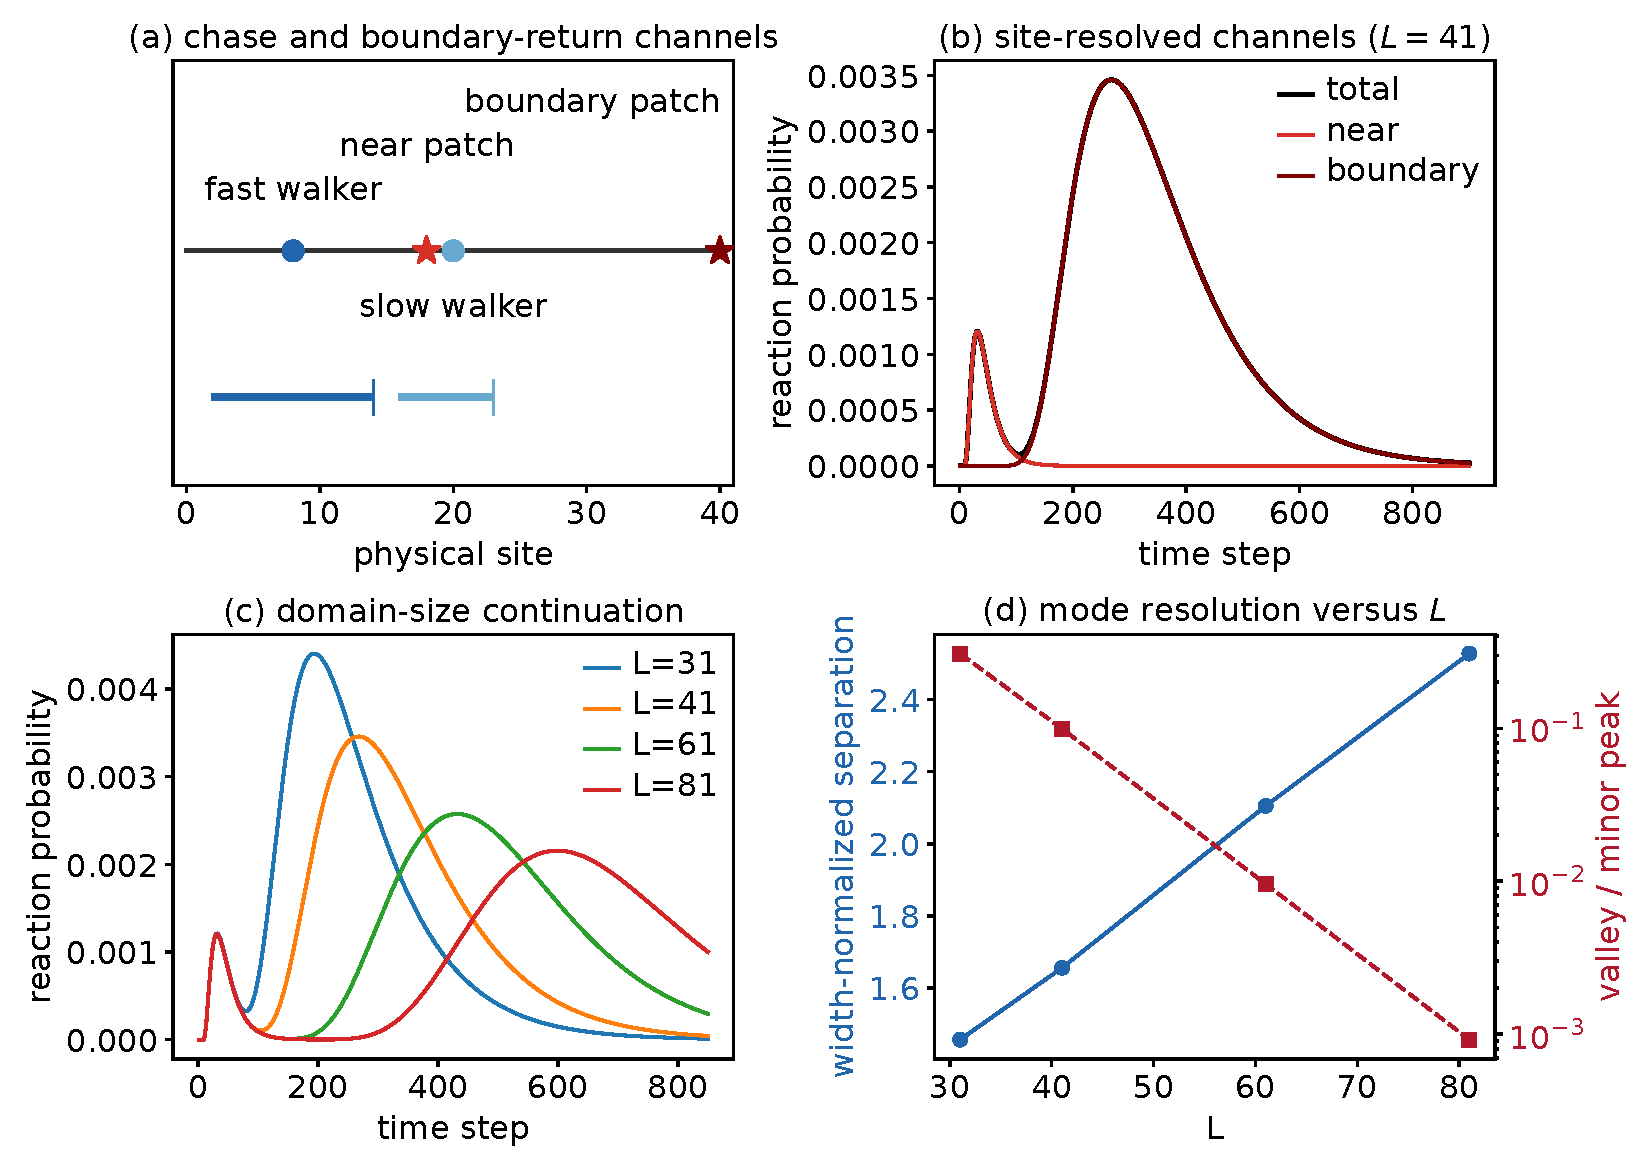
\includegraphics[width=6.65in]{catalytic_encounter_family}
\caption{\label{fig:discovery}
Finite synchronous discovery family. The total reaction-time mass is
resolved into a weak early chase channel at the near catalytic site and a
strong late channel associated with transport to the far site. The early
peak and splitting weight stabilize while the late peak moves with domain
length. The displayed finite-size trends are descriptive evidence, not an
asymptotic theorem.}
\end{figure*}

Poissonization and an independent-clock CTMC retain the two clock windows
(Fig.~\ref{fig:clockcheck}), but they are robustness tests rather than a
calibrated continuous-time limit of the synchronous chain. In particular,
rate and time parameters must not be exchanged between these models.

\begin{figure*}[!t]
\centering
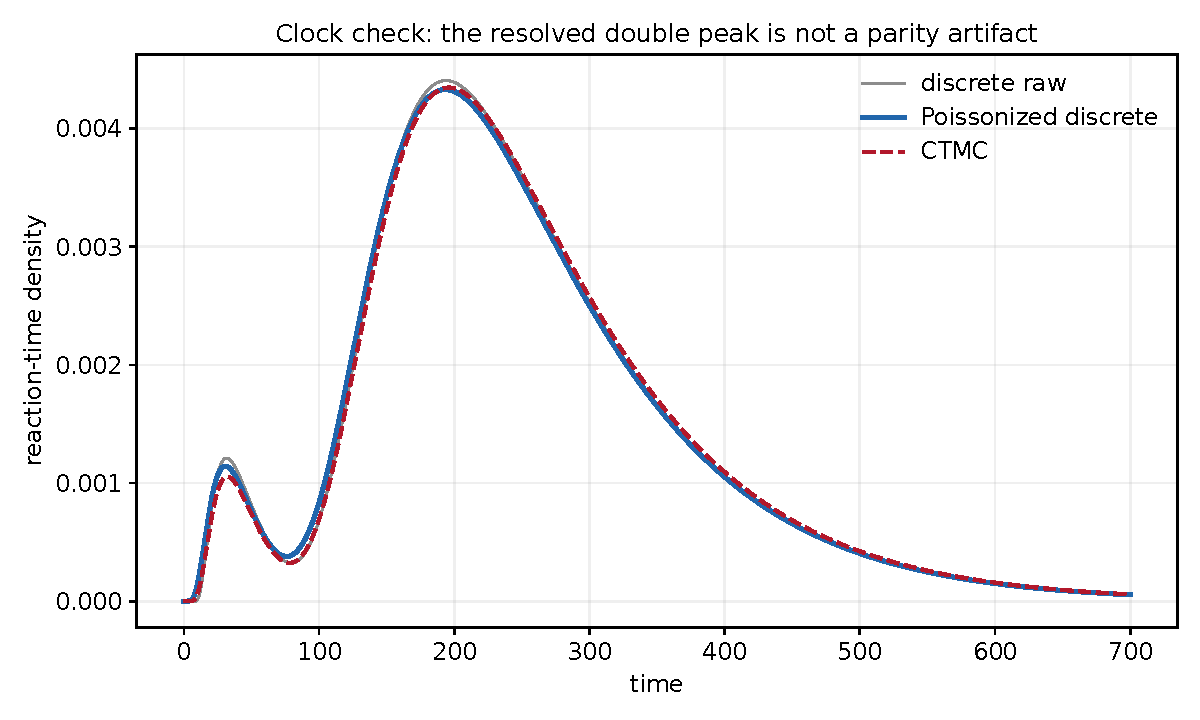
\includegraphics[width=6.65in]{catalytic_encounter_clock_check}
\caption{\label{fig:clockcheck}
Clock robustness. Poissonized synchronous dynamics and an
independent-clock CTMC retain separated early/late windows. The curves test
mechanism robustness under clock changes; they do not establish a calibrated
synchronous-to-CTMC continuum limit.}
\end{figure*}

\subsection{Numerically located finite-CTMC fold}
\label{sec:ctmc-fold}

In the independent-clock \(L=31\) model, we vary
\begin{equation}
\theta=\log(\kappa_{\rm near}/\kappa_{\rm far}),
\label{eq:ctmc-control}
\end{equation}
holding \(\kappa_{\rm far}=0.9162907319\) fixed. Because \(\theta\) changes
both \(T\) and the reaction observable, this is a physical parameter path,
not a freely adjusted mixture weight. The finite-matrix time-derivative
identities follow Eq.~\eqref{eq:time-derivatives}. Parameter derivatives are obtained by
propagating the column state and sensitivity,
\begin{equation}
p'=T^\mathsf Tp,\qquad
s'=T^\mathsf Ts+T_\theta^\mathsf Tp,\qquad s(0)=0,
\label{eq:augmented-sensitivity}
\end{equation}
in one augmented exponential.

The fold occurs at
\begin{equation}
t_*=37.0749586402,\qquad
\theta_*=-9.6753635853,
\label{eq:ctmc-fold-point}
\end{equation}
or \(\kappa_{\rm near}=5.755410148\times10^{-5}\).
Dimensionless first- and second-derivative residuals are
\(7.1\times10^{-15}\) and \(6.8\times10^{-13}\); the dimensionless third
derivative is \(69.94\) and parameter transversality is \(-0.1962\).
Independent points, which were not used to locate the fold, give log--log slopes
\(0.50095\) for critical-point separation and \(1.50877\) for prominence
(Fig.~2 of the main article). The mass-closure error is
\(4.0\times10^{-15}\), and survival at \(t=5000\) is
\(1.3\times10^{-21}\).

For the canonical channel comparison, the joint relative--centre GIG predicts
the early mode at \(26.50\), versus \(32.1534\) for the CTMC, and the
inverse-Gaussian boundary clock predicts \(180.19\), versus \(196.1459\).
The CTMC values are Brent roots of the analytical channel derivative
\(\alpha e^{Tt}Tb_j\), with negative second derivatives, rather than maxima
of a sampled time series.  The relative errors are \(17.6\%\) and \(8.1\%\),
respectively. These
non-negligible errors are reported because no uniform reflected-path
remainder is available. The screening law organizes parameter search; it
does not replace the direct finite-matrix semigroup calculation.

\section{Finite-radius two-dimensional realization}
\label{sec:two-dimensional}

\subsection{Discretization and morphology audit}
\label{sec:2d-method}

The physical domain is the obstacle-free unit square with reflecting outer
boundaries. Each one-particle generator is a conservative boundary-node lattice
CTMC with grid spacing \(L/(n-1)\), central nearest-neighbour diffusion, upwind
longitudinal drift, a smooth transverse restoring drift, and reflection by
omission of outward jumps. This is not a cell-centred finite-volume scheme:
physical \(D,v,\gamma,\kappa\) have dimensions
\(L^2/T,L/T,T^{-1},T^{-1}\), respectively. Length and time are scaled by the
square side \(L\) and a declared time \(T\), and the reported numbers are the
dimensionless groups \(DT/L^2,vT/L,\gamma T,\kappa T\).
The geometric state-sum quadrature assigns equal weights to nodes, and contact
and patch supports are binary node tests. With drift, that equal-node measure
is not the CTMC stationary distribution. Accordingly, the matched catalyst
budget below is an unweighted statewise sum, not a stationary-exposure match.
The free pair generator is the Kronecker sum of the two
one-particle generators. Killing is applied whenever the pair distance is
below the physical reaction radius \(a=0.13\) and the declared midpoint
\(C_{1/2}=(X_1+X_2)/2\) lies inside a catalytic patch.
In the continuum, replacing the open contact and patch disks by their closures
changes only zero-measure boundaries. On every saved lattice, however, both
contact and patch masks use closed ``less-than-or-equal'' tests with a declared
scale-aware floating-point length tolerance. This convention can change binary
state counts at a grid boundary, so those counts and the same closed-mask
convention are retained in the machine artifacts and contact-safe diagnostics.
Bilinear initial weights
preserve physical starting positions across grids, but their independent
product can put artificial mass in the discrete contact tube on a coarse
lattice even when the two physical starts satisfy
\(\lvert x_1^0-x_2^0\rvert>a\). We therefore use the product weights unchanged
when they are contact-safe and otherwise construct a joint initial law by the
nonnegative programme
\begin{equation}
\begin{aligned}
\underset{\alpha_{ij}}{\operatorname{minimize}}\quad
&\sum_{ij}\alpha_{ij}
\bigl(\lvert x_i-x_1^0\rvert^2+\lvert x_j-x_2^0\rvert^2\bigr),\\
\text{subject to}\quad &\sum_{ij}\alpha_{ij}=1,\\
&\sum_{ij}\alpha_{ij}x_i=x_1^0,\\
&\sum_{ij}\alpha_{ij}x_j=x_2^0,\\
&\alpha_{ij}\geq0,\\
&\alpha_{ij}=0\quad\text{if }\lvert x_i-x_j\rvert\leq a+\tau_\ell.
\end{aligned}
\label{eq:contact-safe-initial}
\end{equation}
Here \(\tau_\ell=64\epsilon_{\rm mach}\max(L_x,L_y,a)\) is the
binary64 scale-aware length guard used by the saved contact mask. Patch disks
use the analogous guard with their radius and centre coordinates included in
the maximum. Thus Eq.~\eqref{eq:contact-safe-initial} and the implementation
use the same tolerant closed-support convention.
The smallest feasible expanding local stencil is selected. Because the
minimum-spread linear programme can have a degenerate optimal face, a second,
strictly convex programme selects on that face the unique law closest in
Euclidean norm to the original bilinear product weights; the result therefore
does not depend on an arbitrary linear-programming basis. Physical starts in
the closed contact region are rejected. Saved diagnostics verify unit mass,
nonnegativity, both vector means, zero initial mass on the contact and
active-sink supports, and the root-mean-square and maximum displacement of
each represented start. The coarse-grid solution need not retain independent
marginals; it is the declared minimum-spread, closest-product representation
of two deterministic, noncontacting starts.
Consequently, all results in this section are finite-state mechanism
certificates; no continuum claim is deduced from the boundary discretization.

The principal matched-control family uses
\begin{align}
(D_1,v_1)&=(0.0025,0.18),&
(D_2,v_2)&=(0.0008,0.02),
\label{eq:2d-transport}
\end{align}
transverse confinement \(1.5\), starts
\((0.10,0.50)\) and \((0.35,0.50)\), and patterned reactivity
\begin{equation}
\kappa_{\rm pat}(C_{1/2})=
0.5\,\mathbf 1_{C_{\rm near}}(C_{1/2})
+15\,\mathbf 1_{C_{\rm far}}(C_{1/2}),
\label{eq:patterned-rate}
\end{equation}
with \(C_{\rm near}\) centered at \((0.25,0.50)\), radius \(0.18\), and
\(C_{\rm far}\) centered at \((0.72,0.50)\), radius \(0.20\). The far patch
has positive boundary clearance \(0.08\).

To prevent controls from being mistaken for one-factor ablations, Table
\ref{tab:2d-families} assigns each numerical family an immutable identifier.
All four use \((D_1,D_2)=(0.0025,0.0008)\), transverse confinement $1.5$,
midpoint catalysis, and patch \(y\)-coordinate $0.5$; the entries
\(x/r/\kappa\) specify patch centre, radius, and rate. The families are separate
examples unless an explicit matched path is stated.

\begin{table*}[!t]
\caption{\label{tab:2d-families}Declared bounded two-dimensional model families
and M2D-C branches. Starts list the two initial $x$-coordinates; all initial
$y$-coordinates are $0.5$. The uniform M2D-C row is the unit-domain member of
the separately audited domain-length sweep.}
\begin{ruledtabular}
\begin{tabular}{ccccc}
ID & Role & $a$; starts & $(v_1,v_2)$ & Patches $x/r/\kappa$\\
\hline
M2D-E & matched endpoints & $0.13;\ 0.10,0.35$ & $0.18,0.02$
& $0.25/0.18/0.5;\ 0.72/0.20/15$\\
M2D-F & matched fold & $0.17;\ 0,0.28$ & $0.115,0.02$
& $0.25/0.18/0.5;\ 0.72/0.20/15$\\
M2D-C & separated boundary & $0.13;\ 0.10,0.35$ & $0.18,0.02$
& $0.28/0.12/0.2;\ 0.90/0.20/4$\\
M2D-C & interior two-patch & $0.13;\ 0.10,0.35$ & $0.18,0.02$
& $0.28/0.12/0.2;\ 0.75/0.18/4$\\
M2D-C & single far & $0.13;\ 0.10,0.35$ & $0.18,0.02$
& $0.90/0.20/4$\\
M2D-C & co-located labels & $0.13;\ 0.10,0.35$ & $0.18,0.02$
& $0.90/0.20/0.2;\ 0.90/0.20/4$\\
M2D-C & uniform (unit domain) & $0.13;\ 0.10,0.35$ & $0.18,0.02$
& $0.50/2.00/0.2$\\
M2D-T & three-patch trimodality & $0.13;\ 0.05,0.20$ & $0.10,0.02$
& $0.20/0.06/0.03;\ 0.70/0.05/1;\ 0.94/0.05/0.05$
\end{tabular}
\end{ruledtabular}
\end{table*}

At each grid, a homogeneous rate \(\bar\kappa_h\) is chosen so that
\begin{equation}
\sum_x K_{\rm hom}(x)=\sum_x K_{\rm pat}(x)
\label{eq:budget-match}
\end{equation}
on the same discrete encounter tube. This is an equal per-lattice discrete
state-sum killing budget. It is not equality of every trajectory-level hazard, splitting
probability, or mean lifetime.

For the midpoint coordinate, the change of variables
\(C=(x_1+x_2)/2,\ r=x_1-x_2\) has unit Jacobian.  In the unit square, for
\(0\leq a\leq1\), the exact finite-radius volume of the contact tube is
\begin{equation}
V_T(a)=\int_{|r|\leq a}(1-|r_x|)(1-|r_y|)\,\dd r
=\pi a^2-\frac{8}{3}a^3+\frac12a^4.
\label{eq:finite-a-tube-volume}
\end{equation}
If every catalyst disk has boundary clearance at least \(a/2\), its
centre-space section is untruncated for every admissible \(r\).  The
finite-\(a\) continuum counterpart of Eq.~\eqref{eq:budget-match} is then
\begin{equation}
\bar\kappa_{h,\mathrm{cont}}(a)
=\frac{\pi a^2\,[\pi\sum_j\kappa_j\rho_j^2]}{V_T(a)}.
\label{eq:finite-a-budget-match}
\end{equation}
For M2D-E, \(a=0.13\), both clearances exceed \(a/2\), and
\(\bar\kappa_{h,\mathrm{cont}}=2.169402271\).  The present \(17\times13\)
state-sum rate is \(1.849069451\), still \(14.8\%\) below this reference;
the line in Fig.~\ref{fig:matched} is therefore a finite-radius quadrature
target, not a claim that the five dynamics grids have reached the continuum.

The density is propagated by sparse matrix exponentials on
\(0\leq t\leq80\) with spacing \(0.1\). The audit uses raw and binned
densities, smoothing windows \(1,3,5,9,15\), bin widths
\(1,2,4,8,16\), prominence, lobe mass, valley depth, and persistence across
155 scale views. Survival is propagated separately to \(t=960\), and the
post-window density is searched for additional extrema. The discrete
generator satisfies channel mass balance to \(3.8\times10^{-15}\) or better.
Trapezoidal time integration is used only as a secondary closure diagnostic.

\subsection{M2D-E equal-budget patterned and homogeneous endpoints}
\label{sec:matched-control}

Figure~\ref{fig:matched} compares the M2D-E patterned model with its homogeneous
equal-budget counterpart. The four finer patterned grids are classified
resolved-bimodal, with early peaks \(1.3\)--\(1.5\) and late peaks
\(19.2\)--\(20.8\). The \(9\times5\) patterned grid is a resolved shoulder:
its detected roots, refined by direct finite-matrix semigroup derivative
evaluations, give
strict maxima at \(0.814\) and
\(17.816\), but only one classifier mode. All homogeneous counterparts are
classified resolved-unimodal, with an accepted peak \(1.1\)--\(1.2\). An independent
finite-matrix semigroup derivative audit retains a strict late secondary maximum in
each homogeneous model, but its height is only \(1.02\%\)--\(1.81\%\) of the
primary peak; the patterned secondary/primary ratios are
\(4.43\%\)--\(8.15\%\). A persisted 101-point sweep of the full classifier at
cutoffs strictly inside the unrounded interval
\((1.809905\%,4.434632\%)\) retains every displayed label:
the homogeneous cases remain unimodal, the four finer patterned cases remain
bimodal, and the coarse patterned case remains a shoulder. The interval
endpoints were computed from these same patterned and control realizations,
so this is a post-hoc finite-sample separation audit. It is neither a
predeclared detector range nor an experiment-specific noise-robustness result,
and it is not a continuous-interval theorem.
Repeating the homogeneous control with tensor-product boundary control-volume
budget weights gives strict secondary ratios \(0.637\%\)--\(1.217\%\), zero
two-peak classifier views on every grid, and the same non-bimodal resolution
class (one morphology is a shoulder). Thus the resolution-class contrast is not an artifact of the
state-sum budget measure. Spatial patterning
promotes a subthreshold transport clock to a resolved mode; it is not claimed
to create the mathematical existence of a second local maximum.
The discrete budget mismatch is at most
\(4.2\times10^{-16}\). No post-window maxima are found, and the propagated
tail at \(t=960\) is at most \(1.23\times10^{-10}\) for the patterned family
and \(8.54\times10^{-30}\) for the homogeneous family.
Table~\ref{tab:matched} records the gridwise peak calls and verifies the
state-sum budget equality separately on every lattice; the figure also shows
the control-volume-matched rates.

\begin{figure*}[!t]
\centering
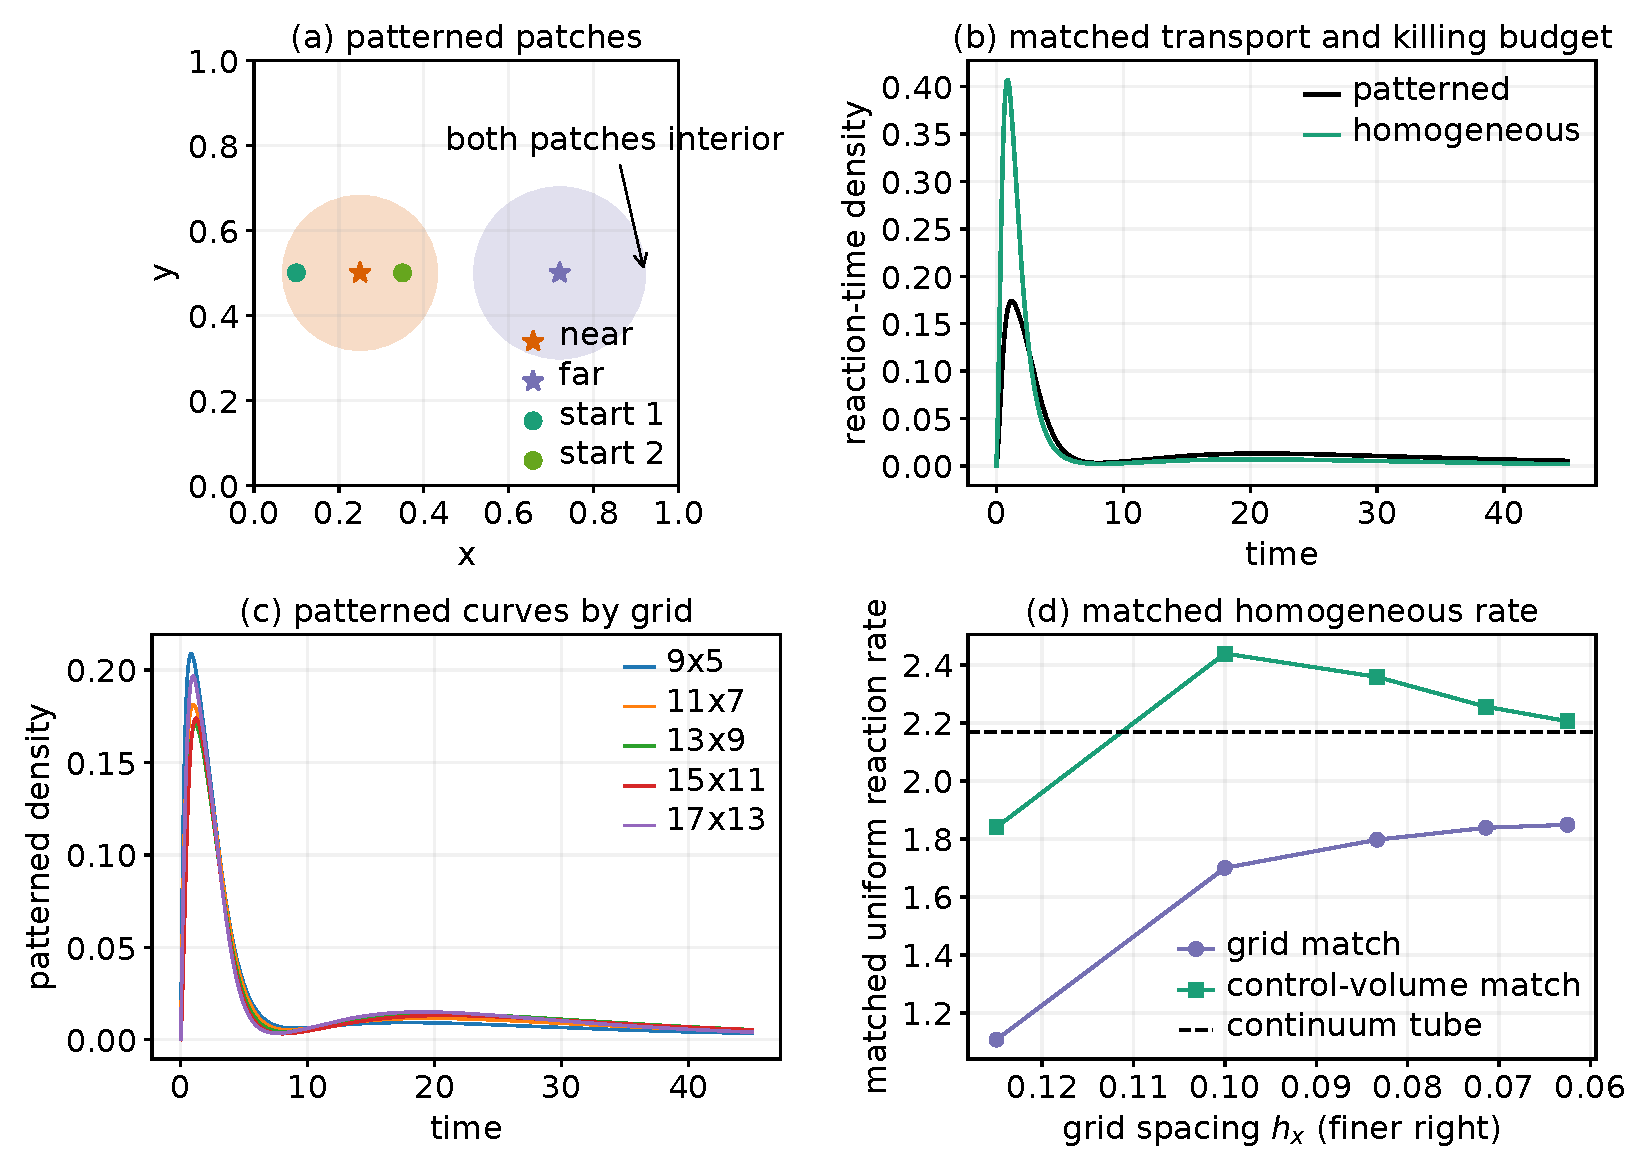
\includegraphics[width=6.65in]{finite_radius_2d_matched_homogeneous}
\caption{\label{fig:matched}
M2D-E finite-radius two-dimensional matched control. At each grid, the patterned
and homogeneous fields have the same sum of statewise killing rates on the
same encounter tube. Homogeneous endpoints are resolved-unimodal on all five
grids; patterned endpoints are resolved-bimodal on the four finer grids and a
resolved shoulder on the coarsest. All strict stationary points, including
the coarse patterned and small homogeneous secondary maxima, are retained
separately. A separate product-control-volume match retains the non-bimodal
homogeneous controls. This establishes finite-grid amplification of a
transport clock under spatial redistribution of a fixed discrete killing
budget; it does not, by itself, locate or prove a continuum fold.}
\end{figure*}

\begin{table*}[!t]
\caption{\label{tab:matched}
M2D-E two-dimensional equal-budget endpoint audit. \(N_+\) is the number of
multiscale views containing two accepted peaks out of 155. The displayed
homogeneous column uses state-sum matching; the control-volume-matched
homogeneous model also has \(N_+=0\) on every grid. ``Strict maxima'' lists
both detected, derivative-refined patterned maxima even when the classifier
calls a shoulder. Each homogeneous model also has a small strict secondary
maximum in the machine artifact; the displayed homogeneous column lists only
the classifier-accepted peak.}
\begin{ruledtabular}
\begin{tabular}{cccccc}
Grid & Patterned call & \shortstack{Patterned strict\\maxima}
& \shortstack{Homogeneous\\accepted peak}
& \shortstack{\(N_+\)\\patterned/homogeneous}
& \shortstack{Relative\\budget error}\\
\hline
\(9\times5\)   & shoulder & \(0.814,\ 17.816\) & \(1.1\) & \(123/0\) & \(4.10\times10^{-16}\)\\
\(11\times7\)  & bimodal & \(0.990,\ 19.518\) & \(1.1\) & \(153/0\) & \(3.08\times10^{-16}\)\\
\(13\times9\)  & bimodal & \(1.142,\ 20.679\) & \(1.1\) & \(155/0\) & \(3.51\times10^{-16}\)\\
\(15\times11\) & bimodal & \(1.191,\ 20.831\) & \(1.2\) & \(155/0\) & \(0\)\\
\(17\times13\) & bimodal & \(0.962,\ 19.061\) & \(1.1\) & \(152/0\) & \(2.23\times10^{-16}\)
\end{tabular}
\end{ruledtabular}
\end{table*}

These are finite-lattice comparisons, not a continuum convergence study. For
M2D-E walker 1, the longitudinal cell P\'eclet number decreases only from
\(9.0\) to \(4.5\), so the upwind effective-diffusion ratio
\(D_{\rm eff}/D=1+\mathrm{Pe}_h/2\) decreases from \(5.5\) to \(3.25\).
Even one transverse cell from the centre on the finest lattice gives local
P\'eclet numbers \(4.17\) and \(13.02\) for walkers 1 and 2. These diagnostics
block an SDE-refinement interpretation while leaving the declared finite CTMC
comparison exact.

\subsection{M2D-F matched-budget fold continuation}
\label{sec:2d-fold-continuation}

For the separate M2D-F family, a natural physical continuation redistributes
its fixed per-lattice state-sum budget,
\begin{equation}
\kappa_\theta(C_{1/2})=(1-\theta)\bar\kappa_h
+\theta\kappa_{\rm pat}(C_{1/2}),\qquad 0\leq\theta\leq1.
\label{eq:2d-budget-path}
\end{equation}
Along this path, both splitting weights and conditional shapes vary.
To resolve the interior fold directly, we use a second declared family with
the same patch geometry and rates but reaction radius \(a=0.17\), walker
parameters \((D_1,v_1)=(0.0025,0.115)\) and
\((D_2,v_2)=(0.0008,0.02)\), and starts \((0,0.5)\) and \((0.28,0.5)\).
The distinction from the endpoint-ablation family above is explicit: the
fold family is a mechanism certificate, not a post hoc claim that every
matched endpoint path has the same critical coordinate. In particular, M2D-F
is not a continuation of M2D-E: its transport parameters, reaction radius,
starts, and per-lattice budget path differ, so neither a common continuation
nor a shared critical coordinate is claimed. On each grid,
\(\bar\kappa_h\) is recomputed from the reactive-state counts, so
\(\sum_xK_\theta(x)\) is constant along \(\theta\) to roundoff.

Sparse generator actions give \(f_t,f_{tt},f_{ttt}\), while an augmented
matrix exponential gives the parameter derivatives. On the
\(9\times5\) grid the fold is
\begin{equation}
(t_c,\theta_c)=(16.8093321,0.27537300),
\label{eq:2d-fold-9}
\end{equation}
with residuals below \(3.5\times10^{-17}\),
\(f_{ttt}=-1.34\times10^{-5}\), and
\(f_{t\theta}=1.67\times10^{-4}\). On the
\(11\times7\) grid the fold is
\begin{equation}
(t_c,\theta_c)=(18.0995323,0.01381035),
\label{eq:2d-fold-11}
\end{equation}
with residuals \((|f_t|,|f_{tt}|)=(8.7\times10^{-19},
3.5\times10^{-18})\), \(f_{ttt}=-7.81\times10^{-6}\), and
\(f_{t\theta}=2.83\times10^{-4}\). On the \(13\times9\) grid,
\begin{equation}
(t_c,\theta_c)=(16.5807587,0.25589201),
\label{eq:2d-fold-13}
\end{equation}
with residuals below \(2.8\times10^{-17}\),
\(f_{ttt}=-5.96\times10^{-6}\), and
\(f_{t\theta}=7.46\times10^{-5}\). Independent continuation gives separation
and prominence exponents \((0.4989,1.5001)\), \((0.4933,1.4843)\), and
\((0.4993,1.5039)\), respectively. Thus all three finite generators verify the
nondegenerate normal form. They are three separate finite-model mechanism
certificates, not a convergent refinement sequence or an estimator of a
continuum critical control.

The state-count-matched critical controls span \(0.262\) and are nonmonotone.
As a one-factor budget-measure audit, we replace equal node weights by the
tensor-product boundary trapezoidal weights on the four-dimensional
two-walker domain, without changing the CTMC generator or reaction masks.
The three nondegenerate folds persist at
\(\theta_c=0.6244,0.2408,0.4593\), but remain nonmonotone and span \(0.384\).
The M2D-F clearances \(0.070\) and \(0.080\) are slightly below
\(a/2=0.085\), so Eq.~\eqref{eq:finite-a-budget-match} is not exact for this
family. Direct one-dimensional quadrature of the boundary-clipped midpoint
sections gives \(\bar\kappa_{h,\mathrm{cont}}=2.2501572\); the factorized
interior-patch counterfactual is \(2.2502051\), a relative difference of only
\(2.13\times10^{-5}\). The weighted homogeneous rates lie closer to the
clipped reference, yet their fold sensitivity confirms that neither sequence
estimates a continuum critical value.

The two even grids clarify the observed topology without supplying a
root-count theorem. On \(12\times8\), a nondegenerate continuation root occurs
at \((t_c,\theta_c)=(18.26877,-0.06158)\), outside the physical interval.
On \(10\times6\), a declared scan of the \(f_{tt}=0\) branches over
\(t\in[0.01,40]\), \(\theta\in[-0.2,0.1]\), followed by four bounded
least-squares starts, finds no fold; every optimizer reaches the same positive
near miss with \(f_t=3.8721\times10^{-6}\). This is only ``no root found under
the declared search,'' not proof of absence.

A separate endpoint audit on
\(9\times5,10\times6,11\times7,12\times8,13\times9\) grids retains every
detected sign-changing stationary point and calls a secondary maximum
resolved only if its height exceeds \(3\%\) of the primary peak and its
intervening valley is below \(95\%\) of the smaller maximum. The finite scan
does not certify the absence of tangential or narrower roots between sampled
times. All homogeneous endpoints are
resolved-unimodal and all patterned endpoints are resolved-bimodal. The two
even grids contain homogeneous reflection ripples below the declared
resolution threshold; these roots are reported rather than deleted. All ten
endpoint tails at \(t=480\) are below \(1.9\times10^{-6}\).
The fixed-budget path, endpoint audit, finite-grid tangencies, and independent
normal-form scaling are collected in Fig.~3 of the main article and are not
duplicated here.

\subsection{Catalytic-coordinate sensitivity}
\label{sec:2d-coordinate-sensitivity}

Equation~\eqref{eq:ceta-relation} shows that midpoint catalysis and the
diffusion-decoupling coordinate define different sinks when $D_1\ne D_2$.
We therefore repeat the M2D-E patterned endpoint calculation with only

\begin{equation}
\eta:\frac{1}{2}\longrightarrow\frac{D_2}{D_1+D_2}=0.242424\ldots
\label{eq:coordinate-control}
\end{equation}

changed. Since this alters the discrete patch support and its raw state-sum
budget, the homogeneous control is rematched independently within every
$(\text{grid},\eta)$ pair. All six homogeneous controls remain
resolved-unimodal under the same canonical threshold; small strict secondary
maxima are retained by the derivative audit. The
midpoint and weighted patterned labels are respectively shoulder/shoulder on
$9\times5$, bimodal/bimodal on $11\times7$, and bimodal/bimodal on
$13\times9$. Near-patch mask Jaccard distances are $0.2222$, $0.1000$,
and $0.2295$; far-patch distances are $0.1000$, $0.0769$, and $0.1493$.
Thus the catalytic coordinate is an observable model convention, not a
relabeling. Label agreement is not model equivalence: the masks and densities
differ on every grid. The finest two comparisons support persistence of the
bimodality mechanism under this diagnostic change, but the coarse shoulder,
nonmonotone masks, and short sequence preclude a continuum-robustness claim.

A supplemental $13\times9$ M2D-T calculation remains three-mode for both
coordinates even though its three patch-mask distances are $0.556$, $0.333$,
and $0.500$. This check is reported separately and does not merge the two
physical models.
Figure~\ref{fig:2d-coordinate} displays the one-factor mask and morphology
sensitivity audit.

\begin{figure*}[!t]
\centering
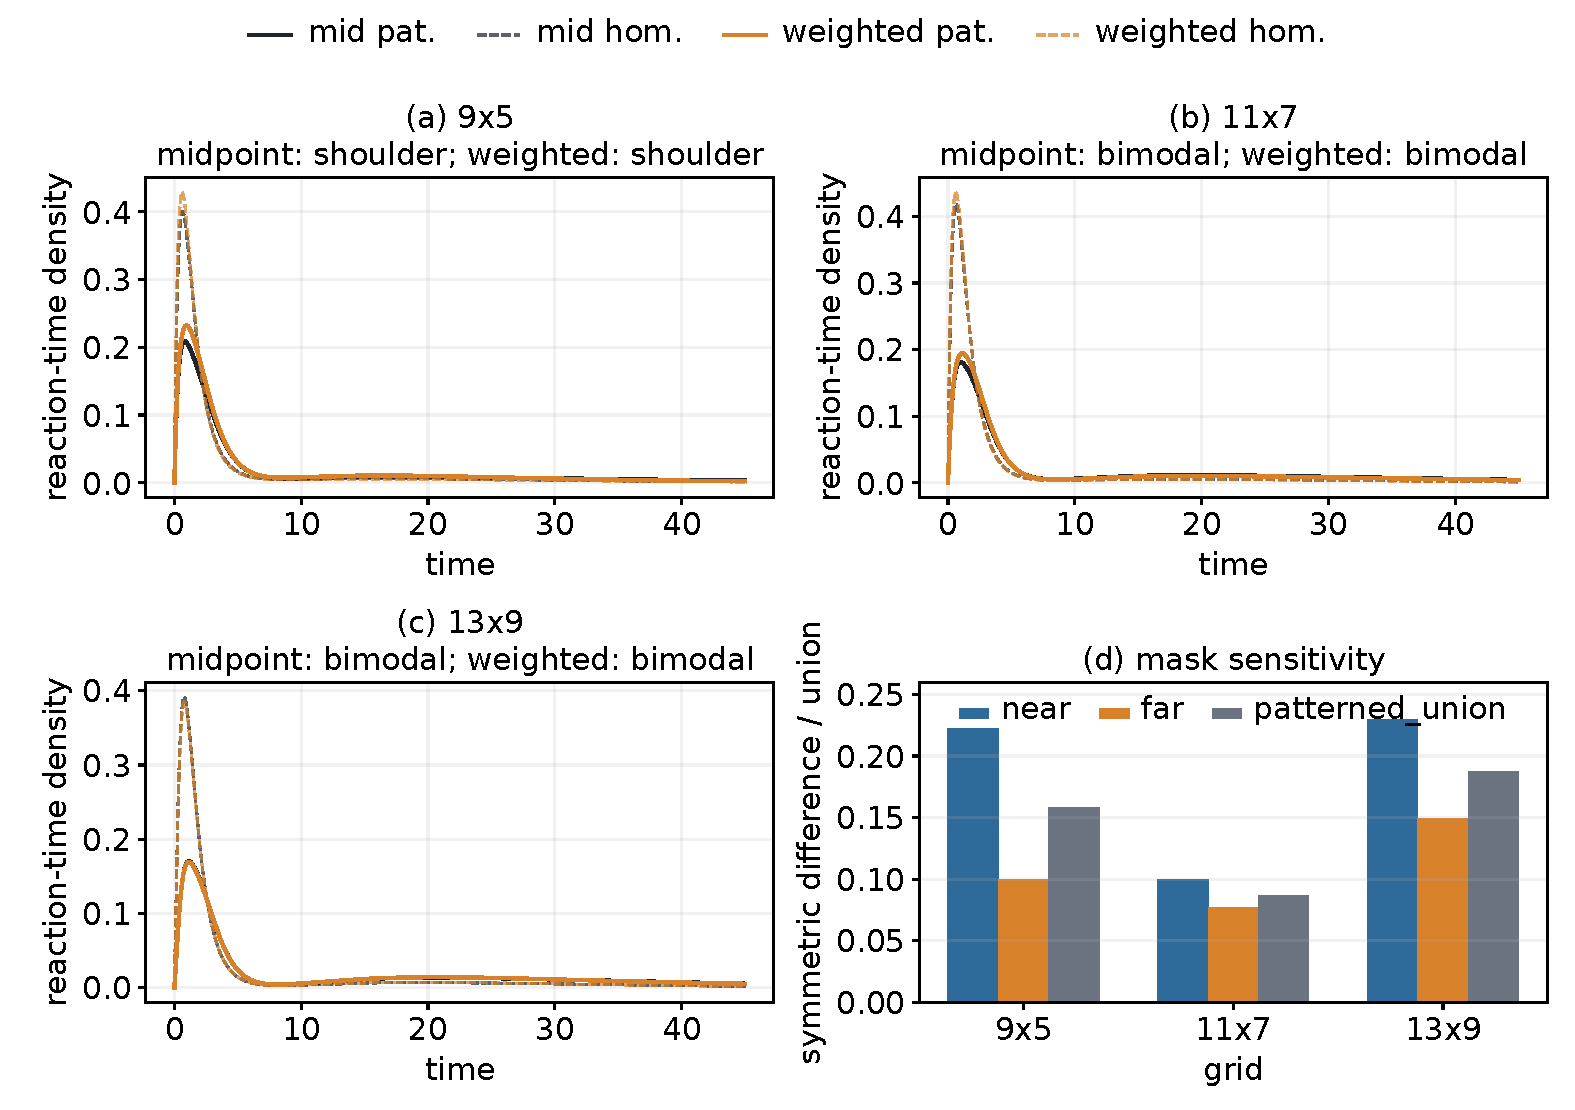
\includegraphics[width=6.65in]{finite_radius_2d_centre_coordinate_sensitivity}
\caption{\label{fig:2d-coordinate}
Catalytic-coordinate sensitivity. The physical midpoint and the
diffusion-decoupling weighted coordinate produce different finite-state patch
masks and densities. Both conventions give a shoulder on the coarsest grid
and bimodality on two finer grids; every within-coordinate budget-matched homogeneous control is
resolved-unimodal under the declared classifier.
This is a finite-grid sensitivity audit, not evidence that the two models are
equivalent in a continuum limit.}
\end{figure*}

\subsection{Interior and adverse controls}
\label{sec:2d-controls}

The separately declared M2D-C examples in Fig.~\ref{fig:controls} illustrate
spatial reaction selection and transport clocks. They change the patch
geometry and rates listed in Table~\ref{tab:2d-families} and therefore are not
factorial one-parameter ablations of M2D-E or M2D-F. Removing the near patch
within M2D-C gives a resolved-unimodal single-far case. Co-locating the two
channel labels at the far position is also resolved-unimodal, showing that
two labels are not sufficient for a resolved second mode. Direct finite-matrix
semigroup derivative evaluations retain a shallow strict max--min--max pattern in both controls;
the second peak fails the scale-persistence and valley-depth criteria (not the
standalone prominence threshold). Moving the far
patch to centre \(x=0.75\), radius \(0.18\), leaves a strictly positive
clearance \(0.07\); the resulting family remains bimodal on the
\(9\times5\) through \(15\times11\) grids. This is a non-touching interior
control, not proof that the reflecting wall is dynamically irrelevant:
late trajectories can still visit the wall.

Most importantly, a separate spatially uniform reactivity
\(\kappa=0.20\) is bimodal on the \(11\times7\) grid, with accepted peaks
near \(1.3\) and \(24.0\). Domain-length scans keep the early peak near one
and move the late peak linearly; the fitted late-peak slope times the slow
drift is \(0.983\), which is consistent with a first-pass/boundary-return
interpretation. This scaling fit is descriptive over the finite
\(0\leq t\leq160\) window: the \(L_x=3\) survival is still \(0.152\) at its
endpoint. A separate post-window audit propagates every domain-scan member to
\(t=480\), where the maximum survival is below \(6.8\times10^{-9}\). On the declared
\(0.25\)-spaced audit mesh, direct finite-matrix derivative observables satisfy
\(f_t<0\) and \(f_{tt}>0\), with no detected post-window stationary point.
This closes the stated tail gate but is neither an interval-exhaustive root
proof nor a pathwise clock decomposition. Thus bimodality persists under
uniform reactivity, and reaction patterning is not necessary. The matched result in
Sec.~\ref{sec:matched-control} consequently supports the restricted statement
that \emph{spatial redistribution of a fixed budget can promote a subthreshold
transport clock into a resolved mode in the stated family}. It does not
support a universal necessity claim or creation of a previously nonexistent
strict extremum.

\begin{figure*}[!t]
\centering
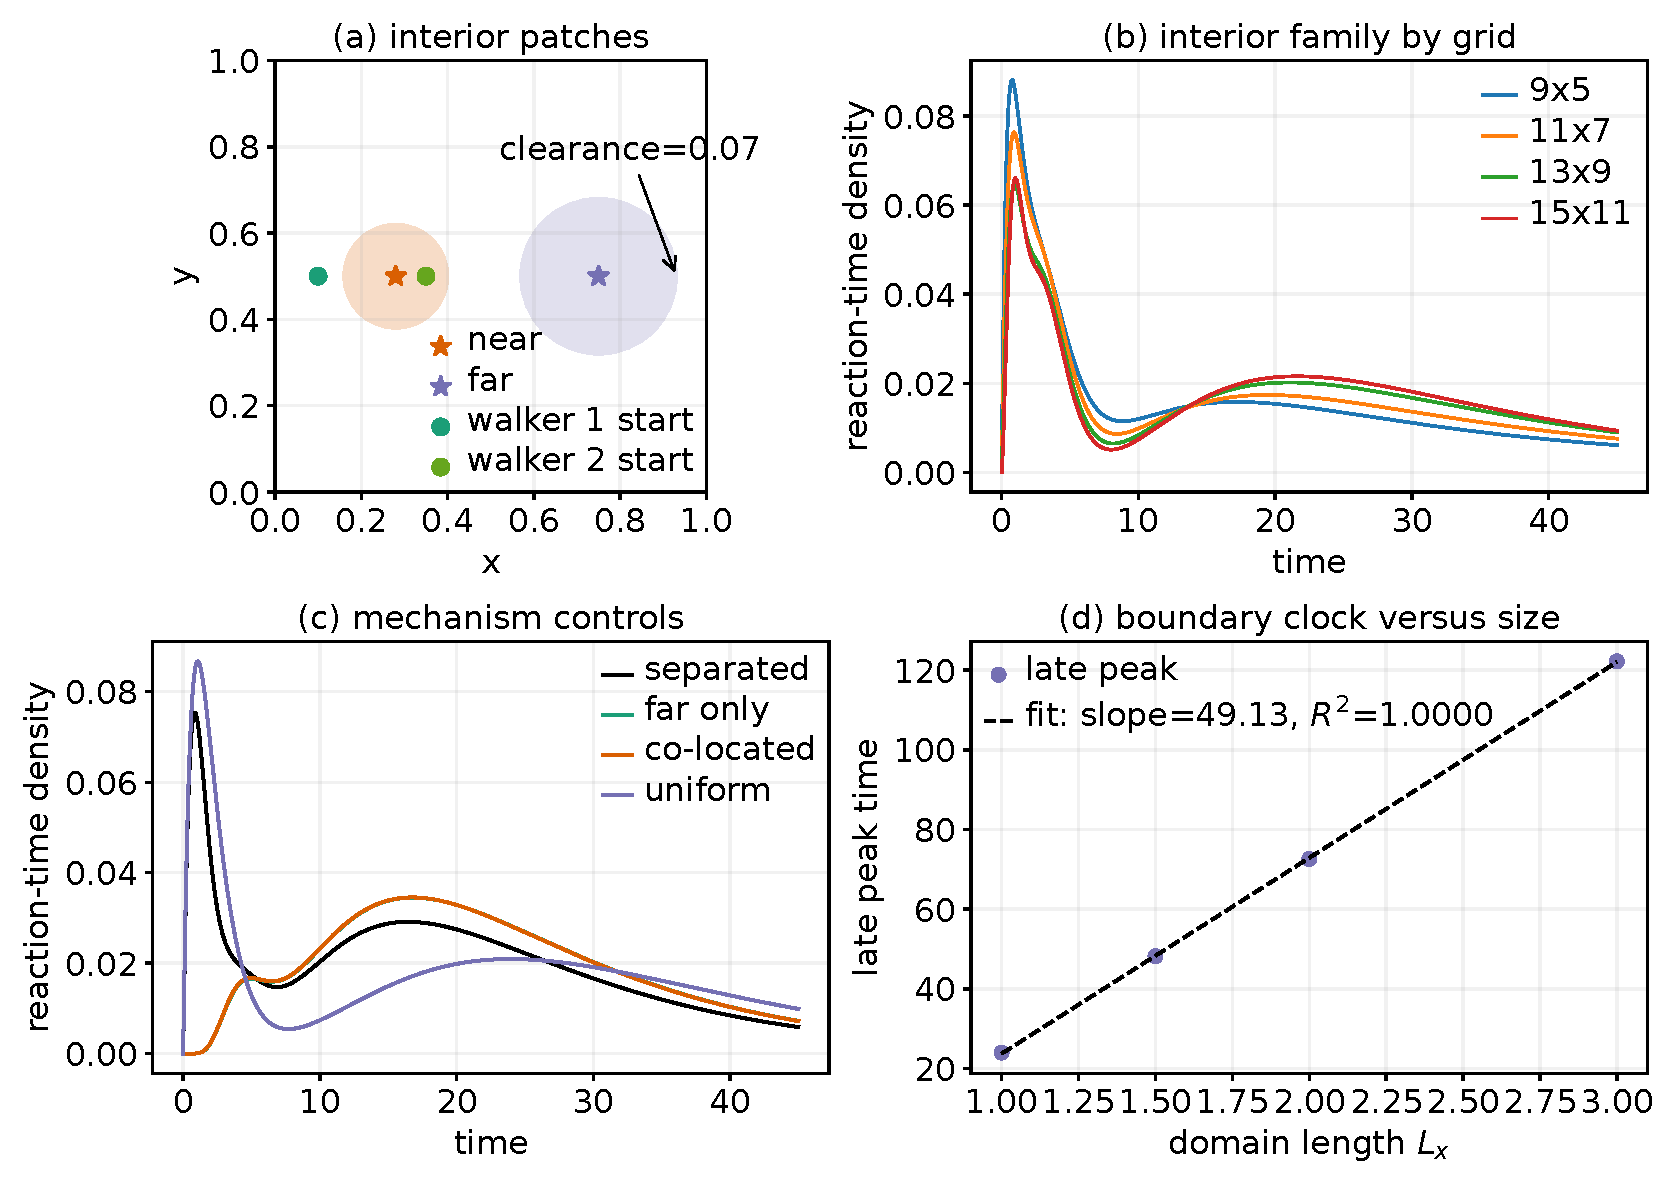
\includegraphics[width=6.65in]{finite_radius_2d_mechanism_controls}
\caption{\label{fig:controls}
Separate mechanism examples in the finite-radius two-dimensional model. The
non-touching interior two-patch family remains resolved-bimodal; single and
co-located reaction opportunities are resolved-unimodal despite retained
shallow strict extrema. A different uniformly reactive model is bimodal, with
its descriptive domain-length scaling consistent with a first-pass and
boundary-return interpretation. A separate tail and finite-matrix derivative
audit through \(t=480\) finds no later stationary point, but is not
interval-exhaustive. These are M2D-C examples rather than one-factor ablations of the
matched M2D-E family. They fix the causal language: patterning is one
controllable route, not a necessary condition.}
\end{figure*}

\subsection{Three-patch finite-grid trimodality}
\label{sec:2d-trimodal}

The separate M2D-T family tests whether three nonnegative spatial channels can
produce three resolved modes in a bounded finite-radius encounter model. Its
parameters are listed in Table~\ref{tab:2d-families}. Direct channel-flux
dominance associates the three detected maxima, in time order, with the near,
middle, and far patches. Their timing is consistent with short-launch,
advective, and delayed downstream-return interpretations, respectively, but
the calculation does not provide a pathwise occupancy decomposition. The far
disk remains inside the square with clearance $0.01$.
This geometry is deliberately reported as a finite-lattice construction:
the patch radii \(0.06,0.05,0.05\) are smaller than \(h_x\) on all four
lattices. Their near/middle/far reactive-state counts are respectively
\(3/3/2\), \(5/5/3\), \(4/4/3\), and \(18/5/5\); the nonmonotone counts expose
binary-mask aliasing rather than continuum refinement.

On each of the $9\times5$, $11\times7$, $13\times9$, and
$15\times11$ grids, the raw density has three strict maxima. The canonical multiscale
classifier resolves all three on the latter three grids; on $9\times5$ it
retains many three-peak scale views but makes the conservative one-mode
``shoulder'' call. Independently, the exact finite-state identity

\begin{equation}
f^{(j)}(t)=\alpha e^{Tt}T^j b
\label{eq:2d-trimodal-derivatives}
\end{equation}

is used to scan $f_t$ to $t=2000$ and refine every sign-change bracket.
The declared scan detects five simple sign-changing roots on each grid,
establishing at least five positive-time roots in the alternating order
maximum--minimum--maximum--minimum--maximum (Table~\ref{tab:2d-trimodal}).
Here ``detected'' is essential: the finite sign-change scan and off-root
logarithmic-slope diagnostic do not constitute an interval-certified exclusion
of an additional tangential root or unresolved narrow root pair. The three
resolved maxima themselves, their intervening minima, and their channel
attribution do not rely on such an exhaustiveness claim.
At the three maxima the dominant flux channels are, in order, near, middle,
and far, with minimum dominant share $0.721$. The maximum absolute root
residual is $1.73\times10^{-15}$, the smallest raw adjacent prominence is
$0.124$ relative to the primary peak, and the largest remaining survival at
$t=2000$ is $4.20\times10^{-11}$.

\begin{table*}[!t]
\caption{\label{tab:2d-trimodal}The five listed positive-time detected
sign-changing derivative roots for the M2D-T family establish at least five
roots on each grid. Each maximum column is dominated respectively by the near,
middle, and far Doi flux; the finite scan is not interval-exhaustive.}
\begin{ruledtabular}
\begin{tabular}{ccc}
Grid & maxima & intervening minima\\
\hline
$9\times5$ & $1.122294,\ 8.554300,\ 34.329213$ & $3.701089,\ 17.850451$\\
$11\times7$ & $1.013153,\ 8.264158,\ 38.893714$ & $3.898736,\ 16.798381$\\
$13\times9$ & $1.016730,\ 8.936256,\ 48.281973$ & $4.455170,\ 15.934062$\\
$15\times11$ & $0.854207,\ 9.315094,\ 48.836751$ & $4.951229,\ 15.557974$
\end{tabular}
\end{ruledtabular}
\end{table*}

Figure~\ref{fig:2d-trimodal} shows the five-root alternation and the direct
near/middle/far channel attribution across the four declared finite grids.

\begin{figure*}[!t]
\centering
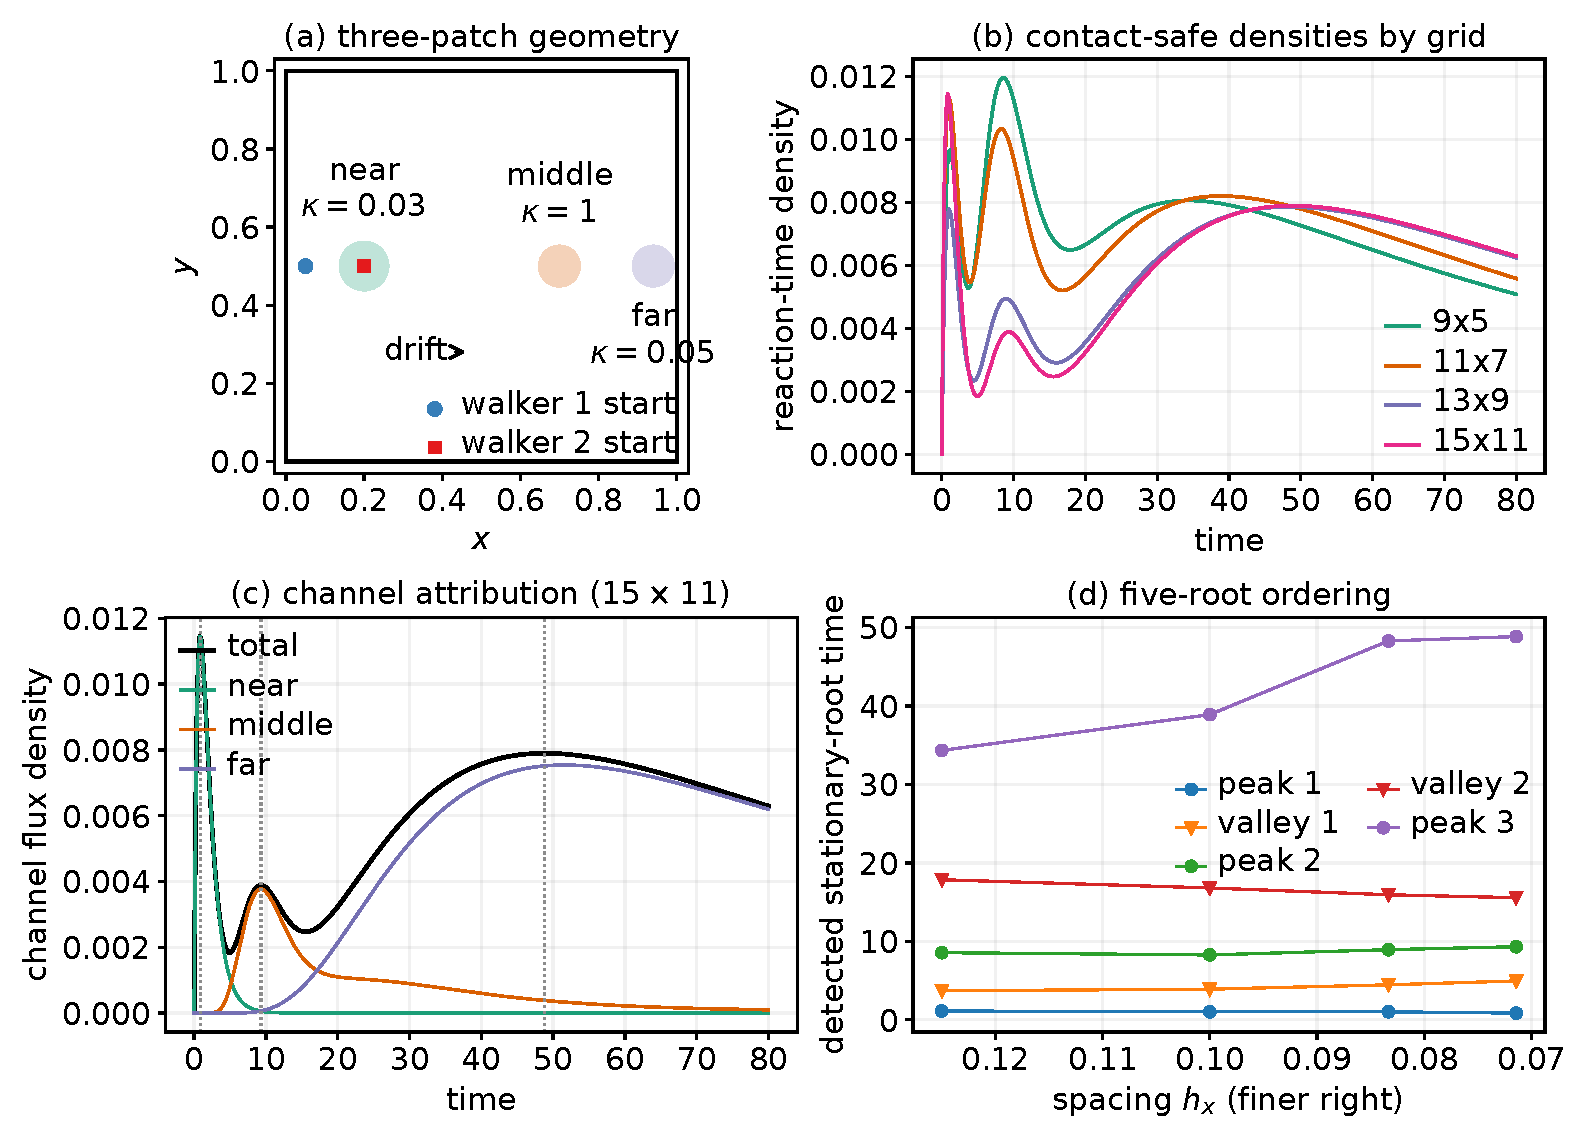
\includegraphics[width=6.65in]{finite_radius_2d_trimodality}
\caption{\label{fig:2d-trimodal}
Finite-radius bounded-domain multi-clock certificate. Three nonnegative
midpoint-selected Doi patches generate three strict maxima on four
boundary-node grids; the classifier resolves all three on the three finer
grids and calls the coarsest a shoulder. Direct finite-matrix semigroup
derivative evaluations detect five alternating sign-changing derivative roots,
thereby establishing at least five positive-time roots, and the three maxima are attributed
directly to the near, middle, and far channel fluxes. The repeated finite-grid
pattern is based on underresolved binary patch masks, and the finite scan is
not interval-exhaustive; it is not a cell-averaged continuum theorem or a
converged trimodality phase boundary.}
\end{figure*}

\section{Capacity-calibrated dimensional extension}
\label{sec:capacity}

Point co-location is not a mesh-independent reaction prescription in physical
dimension \(d\geq2\). The encounter tube has normal dimension \(d\), even
though configuration space has dimension \(2d\). That codimension selects
the small-radius capacity law.

\subsection{Two-dimensional logarithmic capacity}
\label{sec:capacity2d}

Locally in the relative coordinate,
\begin{equation}
G(r,r')\sim-\frac{1}{2\pi\Dr}\log|r-r'|+H
\qquad (d=2),
\label{eq:green-2d}
\end{equation}
so the effective conductance of a small reactive cross-section is
inverse-logarithmic,
\begin{equation}
\keff^{(2)}(a)\simeq
\frac{2\pi\Dr}
{\log[\ell/(a\,\operatorname{cap}_{\log}K)]
 +\beta_{\rm int}+2\pi\Dr H}.
\label{eq:capacity2d}
\end{equation}
For a circular Doi disk with
\(\lambda=a\sqrt{\kappa/\Dr}\), a local intrinsic impedance benchmark is
\begin{equation}
\beta_{\rm int}^{\rm Doi}
=\frac{I_0(\lambda)}{\lambda I_1(\lambda)}.
\label{eq:doi-impedance}
\end{equation}
The domain regular part \(H\), drift, and stationary centre weight cannot be
dropped in the full patterned problem.

To test the normal capacity law without centre heterogeneity, both particles
are placed on the same flat two-torus with translation-invariant reaction.
The pair problem then reduces exactly to a two-dimensional relative process
with diffusivity \(\Dr=D_1+D_2\). At fixed
\(\chi=\kappa a^2/\Dr=1\), the unit-area mean time has leading slope
\begin{equation}
\langle T\rangle
=\frac{1}{2\pi\Dr}\log(1/a)+O(1).
\label{eq:mean2d}
\end{equation}
For grids \(161,241,321,401\), fits over
\(a=0.05,0.04,0.03,0.025,0.02\) give slope ratios to
\(1/(2\pi)\) of \(0.950,0.979,0.984,0.985\), with finest-grid
\(R^2=0.99996\) (Fig.~\ref{fig:capacity2d}). At fixed
\(\kappa=1\), the reaction-limited benchmark
\(\langle T\rangle\sim1/(\kappa\pi a^2)\) is recovered to within
\(0.83\%\) over the tested radii.

\begin{figure*}[!t]
\centering
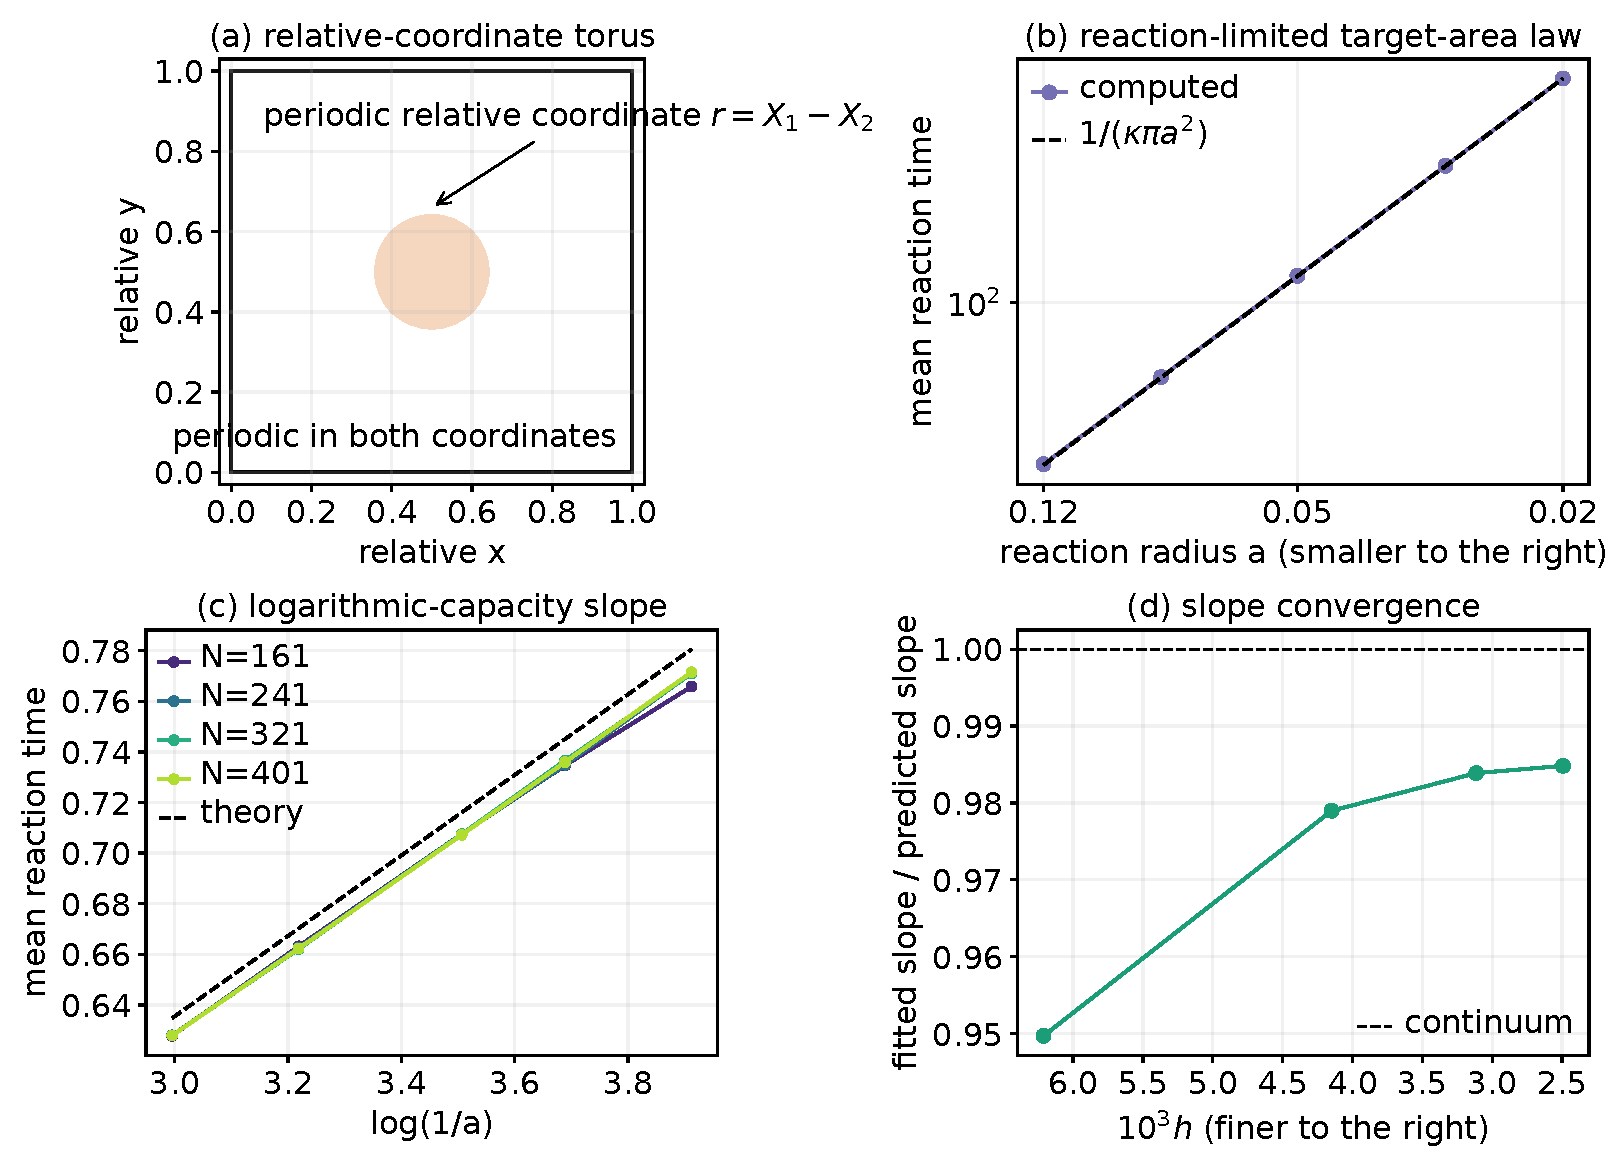
\includegraphics[width=6.65in]{finite_radius_2d_capacity_scaling}
\caption{\label{fig:capacity2d}
Two-dimensional finite-radius calibration on a translation-invariant flat
torus. Fixed-\(\chi\) mean times approach the predicted logarithmic-capacity
slope under grid refinement, while fixed-\(\kappa\) calculations recover the
reaction-limited target-area law. These are relative-coordinate mean-time
benchmarks, not centre-patterned modality calculations.}
\end{figure*}

\subsection{Three-dimensional effective radius}
\label{sec:capacity3d}

In three relative dimensions,
\begin{equation}
G(r,r')\sim\frac{1}{4\pi\Dr|r-r'|}+H.
\label{eq:green-3d}
\end{equation}
For a Doi sphere, matching the regular interior radial solution to the exterior
capture field gives
\begin{equation}
a_{\rm eff}
=a\left(1-\frac{\tanh\sqrt\chi}{\sqrt\chi}\right),
\qquad
\chi=\frac{\kappa a^2}{\Dr},
\label{eq:effective-radius}
\end{equation}
and
\begin{equation}
k_{\rm Doi}^{(3)}=4\pi\Dr a_{\rm eff}.
\label{eq:doi-rate3d}
\end{equation}
On a periodic volume \(V\), the small-target mean has the form
\begin{equation}
\langle T\rangle=
\frac{V}{4\pi\Dr a_{\rm eff}}
+C_{\rm torus}\frac{L^2}{\Dr}
+o(L^2/\Dr).
\label{eq:mean3d}
\end{equation}
The finite-volume correction is additive, so the clean test is the slope
against \(1/a_{\rm eff}\), not equality to the leading term at finite radius.

The matrix-free periodic solver uses cell-averaged Doi spheres, conjugate
gradients, and an FFT inverse of a shifted discrete Laplacian as
preconditioner. Up to \(4.83\times10^6\) states are treated without
assembling the backward operator. Along the coupled fixed-\(\chi\)
radius/grid path, where \(a/h\) stays between about \(7.4\) and \(7.6\), the
smallest-four-radius fit has a slope error \(0.114\%\) relative to
\(1/(4\pi)\). This is continuum-compatible finite-grid evidence, not a
separated double-limit certification. At the separately refined fixed radius
\(a=0.09\), the finest-grid-pair difference is \(0.065\%\), and the largest relative
linear residual is \(6.3\times10^{-14}\). At fixed \(\kappa\),
\begin{equation}
\langle T\rangle\sim
\frac{V}{\kappa(4\pi a^3/3)}
\label{eq:reaction-limited3d}
\end{equation}
is recovered at the smallest radius with \(0.042\%\) relative error.
Figure~\ref{fig:capacity3d} displays the fixed-radius convergence, coupled
capacity path, and reaction-limited cross-check without conflating their
distinct limiting statements.

\begin{figure*}[!t]
\centering
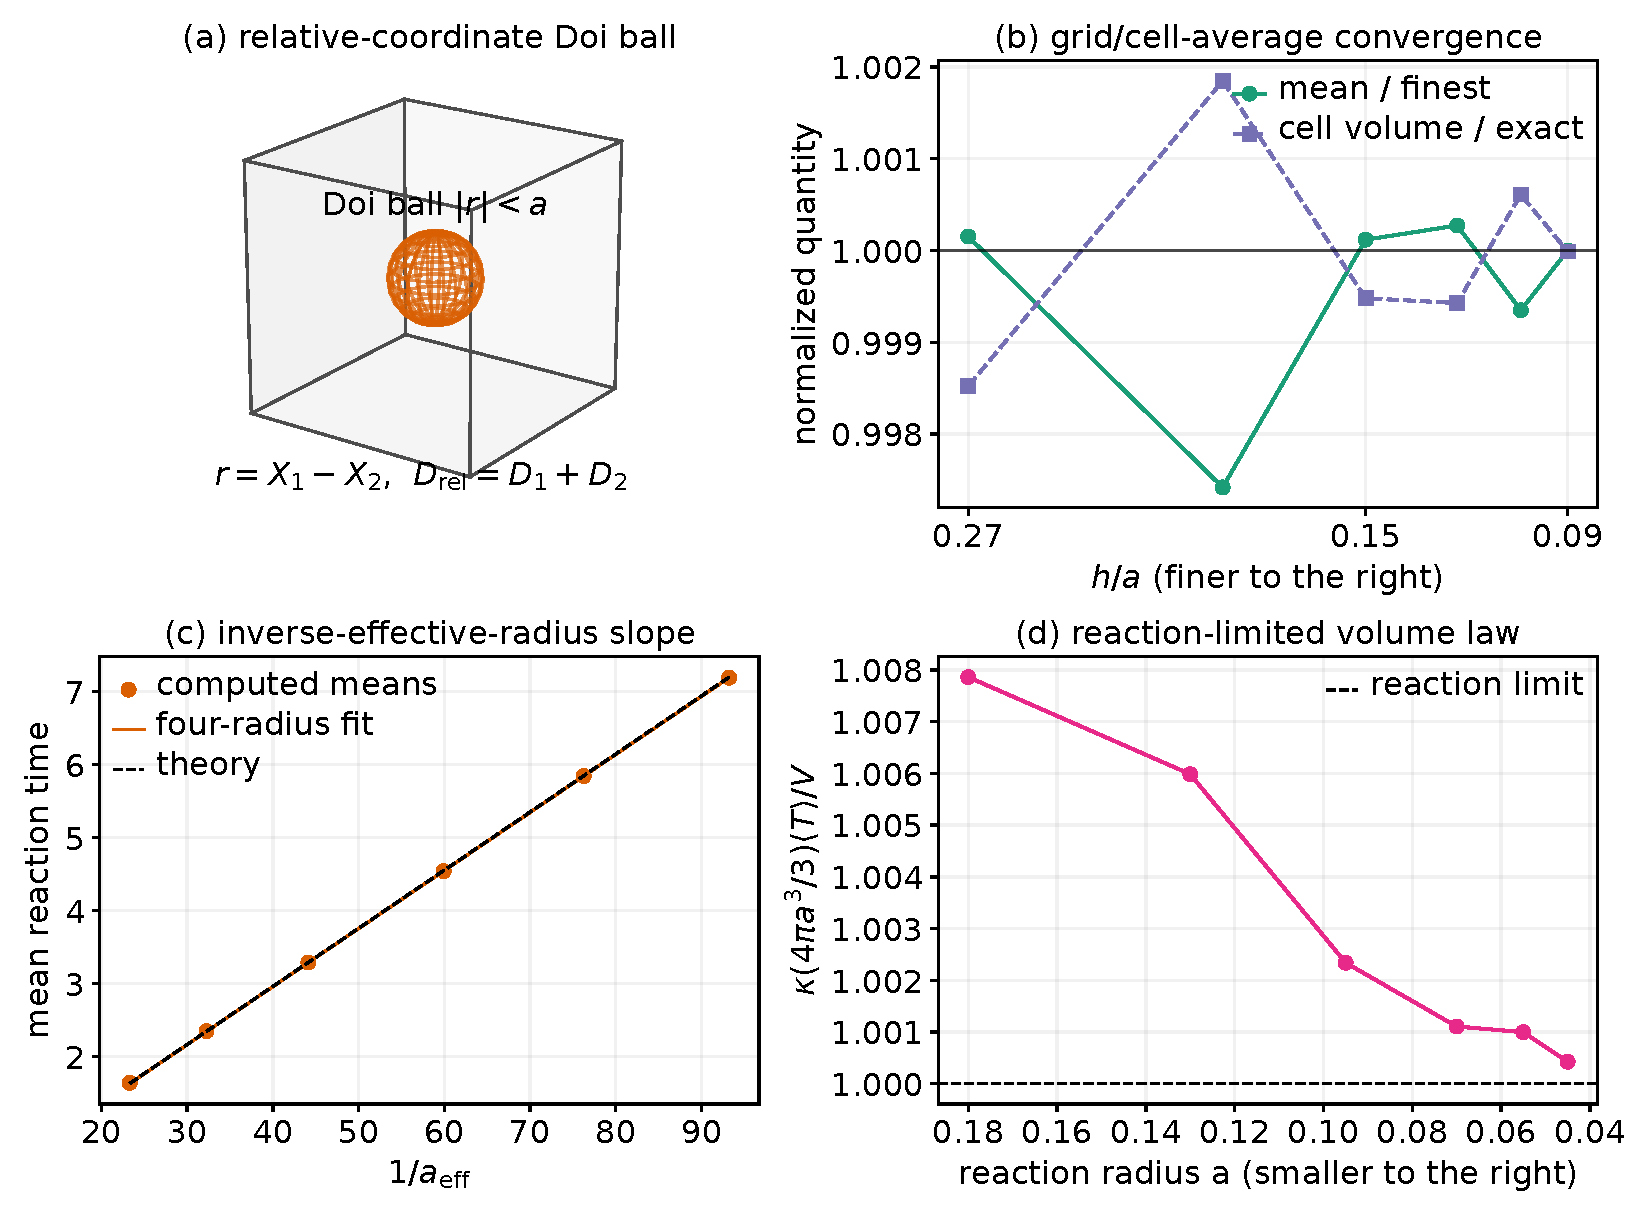
\includegraphics[width=6.65in]{finite_radius_3d_capacity_validation}
\caption{\label{fig:capacity3d}
Three-dimensional Doi capacity on a translation-invariant flat torus.
Fixed-radius grid convergence, coupled-path inverse-effective-radius scaling,
and the fixed-\(\kappa\) reaction-limited law test the relative-coordinate
solver. The radius and grid limits of the shrinking-radius path are not
separately extrapolated. Translation
invariance is essential to the exact quotient; this calculation is not a
six-dimensional centre-patterned modality result.}
\end{figure*}

\section{Additional analyses and analytical obligations}
\label{sec:discussion}

The finite controls distinguish transport-supplied clocks from their
reaction-field weighting; neither transport alone nor heterogeneity alone is a
general explanation. A visible time-domain fold is also not a spectral
exceptional point: poles may be dark or cancelled in the selected observable.

\subsection{Constructive multidimensional screening designs}
\label{sec:multid-design}

The free-space GIG approximation also gives a constructive screening rule for
more than two clocks. In physical dimension \(d\), write
\(p=(d+3)/2\) and use a common \(B>0\). To place the isolated mode of channel
\(j\) at a prescribed time \(m_j\), choose
\begin{equation}
A_j=Bm_j^2+pm_j,
\qquad
w_j=\frac{g_j(m_j)^{-1}}{\sum_k g_k(m_k)^{-1}}.
\label{eq:multid-design}
\end{equation}
The first identity solves the GIG mode equation exactly; the second equalizes
the isolated weighted peak heights without an optimization. For the reference
free-motion mapping \(D_1=D_2=1/2\), initial gap \(\ell=1\), zero relative
drift \(u=0\), and centre speed \(|v_{\mathrm c}|=0.1\), one has \(B=0.01\)
and
\begin{equation}
|z_j-R_0|=\sqrt{Bm_j^2+pm_j-\tfrac14}.
\label{eq:multid-distance}
\end{equation}
More generally the distance is
\(\sqrt{4D_c(A_j-A_{\rm rel})}\), so a real catalyst location requires
\(A_j\ge A_{\rm rel}=\ell^2/(4D_r)\).  In the reference mapping this is
\(Bm_j^2+pm_j\ge1/4\), or
\(m_j\ge[-p+\sqrt{p^2+B}]/(2B)\); the threshold ranges from \(0.12492\)
in \(d=1\) to \(0.071414\) in \(d=4\), below every tested target \(m_j\ge1\).

For dimensions \(d=1,2,3,4\) and target clocks
\((1,10)\), \((1,10,100)\), and \((1,10,100,1000)\), direct isolation of
the analytical derivative roots gives respectively two, three, and four
resolved modes in all 12 tested cases (Fig.~\ref{fig:multid-gig}). The finite
logarithmic scan found \(2m-1\) alternating simple critical points for \(m\)
channels in every case; an interval-certified exclusion of additional
tangential roots is not claimed.
The weakest peak-to-adjacent-valley ratio exceeds \(1.9\), and the largest
scaled derivative residual is below \(2\times10^{-10}\).

This result is a \emph{free-space, narrow-patch GIG screening construction}.
It is not a theorem for a bounded Doi problem. Reflections, finite-patch
averaging, capacity renormalization, and the physical realization of the
designed splitting weights---including compensation for the
time-independent drift cross factors above---remain to be controlled before a three- or
four-mode encounter claim can be made.

\begin{figure*}[!t]
\centering
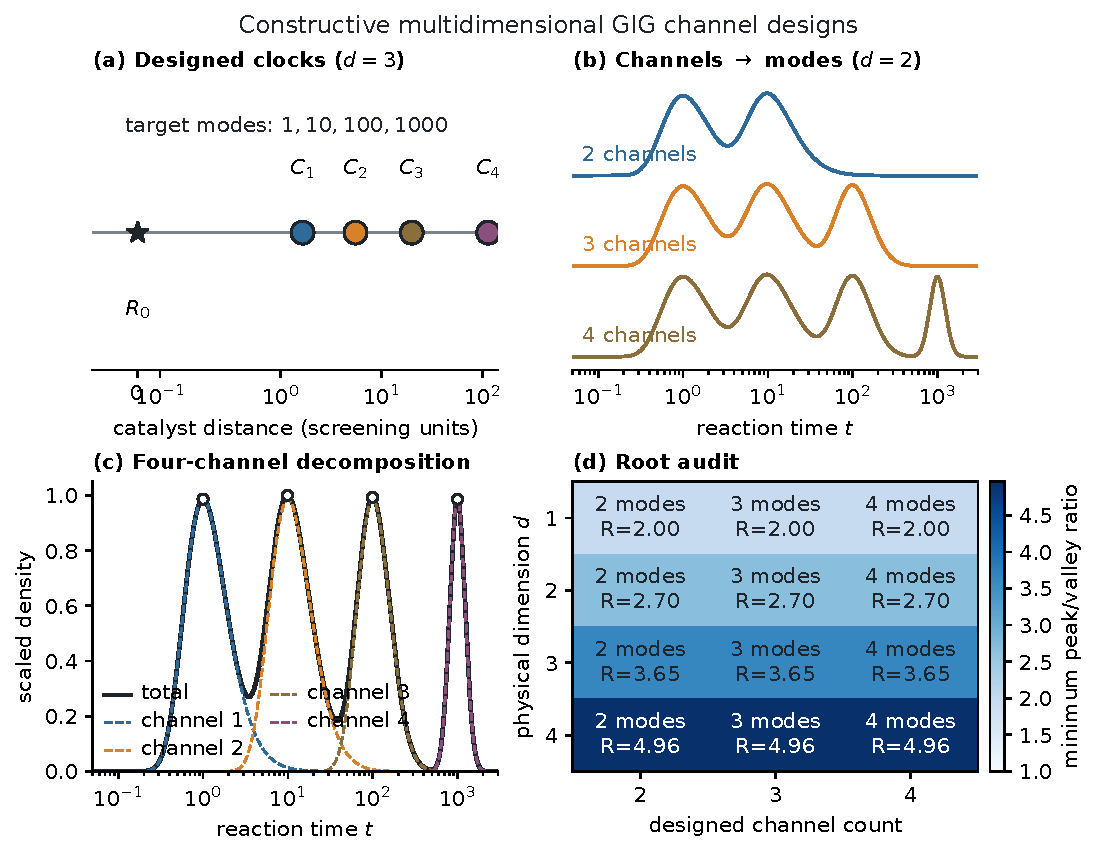
\includegraphics[width=6.65in]{multid_gig_channel_design}
\caption{\label{fig:multid-gig}
Constructive multidimensional GIG channel designs. Prescribed clocks are
mapped to catalyst distances and inverse-isolated-height weights. Analytical
derivatives are numerically root-isolated for two, three, and four channels
in \(d=1,\ldots,4\). The figure validates the declared GIG family only; it is
not evidence for bounded finite-radius Doi trimodality.}
\end{figure*}

\subsection{Relation to prior work}
\label{sec:novelty}

The novelty boundary is deliberately narrow. Confined encounter distributions,
Green and multi-target reductions, heterogeneous reactive locations, GIG
hitting-time laws, capacity asymptotics, and multimodal first-passage densities
are all established. Static heterogeneous bulk killing has already been
optimized at fixed total strength, and partially reactive network elements
have been rearranged at fixed total absorbance
\cite{nguyenGrebenkov2010porous,scottEtAl2021tubular}. Position-dependent
Robin reactivity has also been optimized under a fixed integral constraint to
maximize steady flux \cite{nicolaouMulder2023flux}. Fixed-total-reactivity
spatial optimization is therefore not claimed here. Recent reactive
capacitance theory treats arbitrary patch shapes
\cite{grebenkovMaurette2026capacitance}. In particular, the Brownian
first-passage transition of Besga \emph{et al.} already supplies a
two-time-scale shape change and the merger criterion \(f_t=f_{tt}=0\) under a
target-distance/initial-spread control \cite{besgaEtAl2021dynamical}. It does
not redistribute static Doi reactivity at fixed transport, initial law, and
discrete killing budget, which is the control studied here. The
Giuggioli program already contains multiple peaks generated by periodic-domain
bias, persistence, competing target routes, and small-world disorder, while
resetting and inert heterogeneity reshape peak weights or the location of a
first-passage mode
\cite{sarvaharmanGiuggioli2020biased,dasGiuggioli2022resetting,
marrisGiuggioli2024persistent,barbiniGiuggioli2024heterogeneous,
giuggioliEtAl2024multitarget,marrisEtAl2025disordered}, while Grebenkov showed
that encounter-history-dependent surface activation can induce a
mono-to-bimodal reaction-time change \cite{grebenkov2020paradigm}, and
reactive-state gating can produce multimodal reaction times
\cite{scherReuveni2021unified,scherReuveni2021discrete}.

We use those established propagator, Green, and channel ideas as a
computational layer rather than claiming a new Green theory. The generalized
Descartes rule and Fr\'echet--Duhamel calculus are likewise classical tools;
their mathematical novelty is not claimed. The general increment is to join a
necessary spectral-residue diagnostic to a fixed-budget modality gradient and
test both on the same derivative-certified encounter-fold program. The
spatial evidence then uses two separately declared matched families. M2D-E fixes its
transport generator and discrete state-sum killing budget on each lattice to
test endpoint amplification under spatial redistribution. M2D-F fixes a
different transport generator and its own per-lattice state-sum budget, then
locates a density transition through
\(f_t=f_{tt}=0\) with nondegeneracy and physical-path transversality. The
supporting spatial results are the M2D-E five-grid endpoint audit with four
resolved label contrasts, three nondegenerate but nonconverged M2D-F
finite-grid folds, and a bounded finite-grid three-channel mechanism
certificate. They are not a first
observation of multiple peaks or of a passage-time shape transition, a new
Woodbury identity, or a continuum modality theorem. Static
fixed-total-reactivity design, heterogeneous reaction,
reactivity-generated bimodality, and the Green machinery are not claimed as
new; the model-specific new object is the finite-grid density fold under the
stated M2D-F matched experiment, with M2D-E providing a separate
endpoint-amplification audit. The finite-state local-sensitivity calculus explains which
budget-feasible perturbations can unfold such a boundary without asserting a
continuum optimum.

\subsection{Limitations and analytical obligations}
\label{sec:limitations}

Several limitations are necessary to interpret the results correctly.
\begin{enumerate}
\item The GIG law has no uniform remainder over a mode-containing window and
is not a global reflected-path expansion.
\item The inverse-free continuum Green identity requires operator-domain
hypotheses. The implemented left-half-plane pole/residue and derivative
validations are finite-dimensional; continuum meromorphic continuation is not
established. Near the reflecting zero mode, the free-Green implementation is
fail-closed and the stable zero-frequency quantities use the killed solve.
\item The spectral sign-variation corollary is necessary but not sufficient
and is used only for finite reversible generators with grouped real decay
rates. The primary-model spectra have far more sign changes than the observed
roots, so the count is a falsification gate rather than a mode predictor. It
does not apply unchanged to complex spectra, Jordan terms, or an infinite
continuum expansion.
\item The budget-projected modality gradient is an infinitesimal interior-rate
result. Its closed-form optimizer ignores finite-amplitude nonnegativity, box
constraints, binary patch masks, and the nonsmooth motion of a sharp support.
Those constraints require a separate quadratic, shape, or mixed-integer
design problem.
\item The physical fold is numerically located to the stated tolerances for one
finite CTMC using exact finite-matrix derivative identities; it is not uniform
in lattice spacing, radius, or system size. Its minority splitting probability is
\(8.95\times10^{-6}\). The corresponding absorption law is phase type;
finite-state multimodality is not claimed as a new probability-law class.
\item The M2D-E endpoint and M2D-F fold comparisons use moderate grids and an upwind
Doi discretization. Cell P\'eclet numbers remain large, so the tested lattices
are not a controlled refinement of the displayed continuum SDE. The three
fold controls are nonmonotone, span \(0.262\), and move substantially under a
product-control-volume budget measure. Their location is not grid-converged.
The resolved endpoint contrast is operational: the full classifier is stated,
but no experiment-specific detector or noise model derives its 3\% scale.
An independent Robin solver and Doi--Robin matching are not included.
Even convergence of the density in \(C^2\) would not by itself transfer a
nondegenerate fold; the required target is joint \(C^3\) convergence in time
and control, including the parameter Duhamel derivatives.
\item The bounded 2D model declares midpoint catalysis. The
diffusion-decoupling weighted-coordinate control changes discrete masks and the
quantitative densities even though the three tested morphology labels agree;
no invariance with respect to \(\eta\) or equivalence
of these physical sink models is claimed.
\item Equal per-lattice discrete state-sum killing is one matching rule; it does not match every
pathwise hazard, splitting weight, or mean lifetime. The separate M2D-C
uniform-reactivity counterexample rules out necessity language.
\item The interior far patch has clearance \(0.07\), but late trajectories can
still feel the reflecting boundary. Enlarged-domain or periodic matched
controls are needed before claiming boundary independence.
\item The 2D and 3D capacity studies exploit translation invariance and concern
mean reaction times. They do not prove full centre-patterned channel-density
or modality convergence.
\item Four-size scaling fits are descriptive. Peak separation alone does not
prove a large-distance two-mode theorem; derivative-dominance bounds, weights,
widths, and a controlled remainder are required.
\item The M2D-T family establishes three classifier-resolved finite-grid
trimodal cases and a fourth finite-grid density with three strict maxima but a
classifier shoulder. Each grid has at least five detected sign-changing roots
in the alternating pattern, but the finite scan is not an
interval-exhaustive root certificate and establishes no cell-averaged
continuum trimodal region, converged cusp, or general-\(d\) modality theorem.
Every patch radius is below the longitudinal grid spacing,
and the reactive-state counts are nonmonotone. The multi-channel GIG
construction remains a free-space screening result.
\end{enumerate}

A continuum persistence theorem should decompose
\begin{equation}
f_L=w_{E,L}g_{E,L}+w_{B,L}g_{B,L}+\varepsilon_L
\label{eq:large-separation}
\end{equation}
and control both channels and their first two derivatives in neighborhoods of
the early peak, the late peak after centering and scaling, and the intervening
valley. Nonvanishing limiting weights, nondegenerate channel maxima, and
cross-channel derivative margins would then imply two persistent modes by
stability of simple critical points. Transferring the fold itself additionally
requires the joint \(C^3\) control in Eq.~\eqref{eq:fold-ift-determinant} and
convergence of the budget-projected parameter derivative. Establishing these
assumptions from the encounter generator, rather than fitting peak locations,
is the next analytical step.

\appendix
\renewcommand{\thesection}{S\Alph{section}}
\renewcommand{\thesubsection}{S\Alph{section}.\arabic{subsection}}
\renewcommand{\thesubsubsection}{S\Alph{section}.\arabic{subsection}.\arabic{subsubsection}}
\renewcommand{\theequation}{S\Alph{section}\arabic{equation}}

\section{Fold normal-form prominence}
\label{app:normal-form}

Let
\begin{equation}
F(t,\theta)=f_t(t,\theta)
=a_*\Delta\theta+\frac{b_*}{2}\Delta t^2
+o(|\Delta\theta|+|\Delta t|^2).
\label{eq:app-normal}
\end{equation}
Set
\begin{equation}
c=\sqrt{-\frac{2a_*}{b_*}\Delta\theta}.
\label{eq:app-c}
\end{equation}
At leading order the two new critical points are at
\(\Delta t_\pm=\pm c\). The density difference between the local maximum and
minimum is the integral of \(F\),
\begin{align}
\mathcal P
&=\left|\int_{-c}^{c}
\left(a_*\Delta\theta+\frac{b_*}{2}x^2\right)\dd x\right|\\
&=\frac{2|b_*|}{3}c^3
=\frac{2|b_*|}{3}
\left|-\frac{2a_*}{b_*}\right|^{3/2}
|\Delta\theta|^{3/2},
\label{eq:app-prominence}
\end{align}
up to \(o(|\Delta\theta|^{3/2})\). This gives the \(3/2\) exponent used in
the independent CTMC validation.

\section{Finite-state mass and derivative identities}
\label{app:finite-identities}

For a row generator \(T\), initial row distribution \(\alpha\), and total
killing vector \(b=UK\bm1=-T\bm1\),
\begin{equation}
S(t)=\alpha\e^{Tt}\bm1,\qquad
f(t)=\alpha\e^{Tt}b.
\label{eq:app-survival}
\end{equation}
Therefore
\begin{equation}
-S'(t)=-\alpha\e^{Tt}T\bm1
=\alpha\e^{Tt}b=f(t),
\label{eq:app-mass}
\end{equation}
which is the exact finite-state version of
Eq.~\eqref{eq:mass-balance}. If the killed chain is transient,
\begin{equation}
\int_0^\infty \alpha\e^{Tt}UK\,\dd t
=\alpha(-T)^{-1}UK.
\label{eq:app-splitting}
\end{equation}
Repeated time differentiation yields
Eq.~\eqref{eq:time-derivatives}. For \(T=T(\theta)\), Duhamel's identity gives
\begin{equation}
\partial_\theta\e^{Tt}
=\int_0^t\e^{T(t-s)}T_\theta\e^{Ts}\,\dd s,
\label{eq:app-duhamel}
\end{equation}
which is equivalent to the augmented sensitivity propagation in
Eq.~\eqref{eq:augmented-sensitivity}.

\section{Numerical evidence and provenance boundary}
\label{app:provenance}

The numerical sources are the JSON and CSV artifacts accompanying this
article. Each secondary calculation has a machine-readable manifest recording
the command, source hashes, model specification, runtime, and output hashes.
Before submission, these manifests must be regenerated from a clean tagged
commit and aggregated by a transitive top-level manifest.

The accompanying Lean~4/mathlib package contains 140 theorem/lemma
declarations, including 60 encounter-specific statements. Static source
inspection finds no executable \texttt{sorry}, \texttt{admit}, or declared
axiom. The preserved 2026-07-14 build and theorem-printing logs record a local
build without errors, and the preserved theorem-by-theorem reports list only
\texttt{propext}, \texttt{Classical.choice}, and \texttt{Quot.sound}.
No independent Lean rebuild is claimed here.
The encoded results cover the two-channel fold elimination and quadratic
normal form, the two-hotspot inverse, scalar/componentwise affine-centre
algebra and a one-dimensional absolute-value contact bound, the scalar
relative--centre transform, the GIG stationary-point equation, the pure
\(a^{d-2}\) capacity-power algebra without its geometric constant or a capacity
theorem, finite exponential-mixture derivatives, and inverse-height design
weights. In a general real inner-product design space, it also proves that the
one-budget projected gradient is tangent, preserves every feasible response,
bounds every unit feasible response, and that its normalized nonzero direction
attains the bound. Taking the inner product to be
\(\langle x,y\rangle_M=x^\mathsf TMy\), with Riesz vectors
\(M^{-1}c\) and \(M^{-1}g\), gives Eqs.~\eqref{eq:budget-projection} and
\eqref{eq:optimal-redistribution}. The prescribed-action results prove
vanishing log derivative at the chosen time, not formal uniqueness or
maximality of that stationary point.
This formal build certifies only
those algebraic implications. It does not certify PDE regularity,
floating-point roots, grid or continuum limits, or the applicability of the
encoded assumptions to the physical model.

\section{Proof of the fold-transfer theorem}
\label{sm:fold-transfer-proof}

Write \(q=(t,\theta)\), \(H(q)=(F_t,F_{tt})(q)\),
\(H_h(q)=(F_{h,t},F_{h,tt})(q)\), \(J=DH\). The four entries of \(J\)
admit the augmented modulus \(\hat\omega(r)=\max(\omega(r),\sqrt2\Lambda r)\):
the entry \(F_{tt}\) is
\(\sqrt2\Lambda\)-Lipschitz (its gradient is \((F_{ttt},F_{tt\theta})\),
bounded entrywise by \(\Lambda\)), and \(F_{t\theta},F_{ttt},F_{tt\theta}\)
carry \(\omega\) by hypothesis, so each entry of \(J(q)-J(q')\) is at most
\(\hat\omega(\|q-q'\|)\), and \(\hat\omega(r_0)\le\hat\omega(r_\omega)\le
\sigma/16\) by the (nondecreasing) definition of \(r_\omega\). For a
\(2\times2\) matrix with entries bounded by \(\hat\omega\), the operator
norm is at most \(2\hat\omega\); we use this factor explicitly. All norms are
Euclidean and induced operator norms, and \(B(q_*,r_0)\subseteq N\) by the
definition of \(r_0\).

\emph{Step 0 (seed conditioning).} At \(q_*\), \(F_{tt}=0\),
\(|F_{ttt}|\ge\mu_3\), and \(|F_{ttt}|,|F_{tt\theta}|\le\Lambda\), so
\[
\sigma=\sigma_{\min}(J(q_*))
=\frac{|\det J(q_*)|}{\sigma_{\max}(J(q_*))}
\ge\frac{|F_{t\theta}|\,\mu_3}{\sqrt{F_{t\theta}^2+2\Lambda^2}}
\ge\frac{\mu_3\mu_\theta}{\sqrt{\mu_\theta^2+2\Lambda^2}},
\]
using \(\sigma_{\max}\le\|J\|_F=\sqrt{F_{t\theta}^2+F_{ttt}^2+F_{tt\theta}^2}\)
and monotonicity of \(x\mapsto x/\sqrt{x^2+2\Lambda^2}\).

\emph{Step 1 (perturbation inventory).} The defect matrix \(DH_h-DH\) has
entries bounded by \(\varepsilon_h\) (entry \(F_{tt}\)) and
\(\varepsilon_h'\) (entries \(F_{t\theta},F_{ttt},F_{tt\theta}\)), so
\(\|DH_h-DH\|\le\sqrt{\varepsilon_h^2+3\varepsilon_h'^2}
\le2\bar\varepsilon_h\). By \(\hat\omega(r_0)\le\sigma/16\),
\(\|J(q)-J(q_*)\|\le2\,\hat\omega(r_0)\le\sigma/8\) on \(B(q_*,r_0)\).

\emph{Step 2 (simplified Newton).} Assume
\(\bar\varepsilon_h<\delta_0\le\sigma/32\), so
\(2\bar\varepsilon_h\le\sigma/16\) and \(4\bar\varepsilon_h\le\sigma/8\).
At the seed,
\(\|DH_h(q_*)-J(q_*)\|\le2\bar\varepsilon_h\le\sigma/16\), so by the
Neumann series
\(\|DH_h(q_*)^{-1}\|\le\tfrac{16}{15}\|J(q_*)^{-1}\|
\le\tfrac87\|J(q_*)^{-1}\|\). Define
\(\Phi(q)=q-DH_h(q_*)^{-1}H_h(q)\). For \(q\in B(q_*,r_0)\),
\[
\|D\Phi(q)\|
=\|DH_h(q_*)^{-1}\big(DH_h(q_*)-DH_h(q)\big)\|
\le\frac87\cdot\frac1\sigma\Big(2\,\hat\omega(r_0)+4\bar\varepsilon_h\Big)
\le\frac87\cdot\frac1\sigma\cdot\frac{\sigma}{4}=\frac27 ,
\]
since
\(\|DH_h(q_*)-DH_h(q)\|\le\|(DH_h-DH)(q_*)\|+\|DH(q_*)-DH(q)\|
+\|(DH-DH_h)(q)\|\le2\bar\varepsilon_h+2\hat\omega(r_0)+2\bar\varepsilon_h\).
Also \(\|\Phi(q_*)-q_*\|=\|DH_h(q_*)^{-1}H_h(q_*)\|\le\alpha\) with
\(\alpha:=\tfrac{8\sqrt2}{7}\|J(q_*)^{-1}\|\varepsilon_h\), because
\(\|H_h(q_*)\|=\|(H_h-H)(q_*)\|\le\sqrt2\,\varepsilon_h\). The fourth term
of \(\delta_0\) gives
\(\tfrac75\alpha=\tfrac{8\sqrt2}{5\sigma}\varepsilon_h\le r_0\), so
\(\Phi\) maps \(B(q_*,\tfrac75\alpha)\subseteq B(q_*,r_0)\) into itself
(\(\alpha+\tfrac27\cdot\tfrac75\alpha=\tfrac75\alpha\)) and is a
\(\tfrac27\)-contraction there. The Banach fixed point \(q_h\) satisfies
\(H_h(q_h)=0\) and
\[
\|q_h-q_*\|\le\frac{\alpha}{1-\tfrac27}
=\frac75\alpha
=\frac{8\sqrt2}{5}\,\|J(q_*)^{-1}\|\,\varepsilon_h
\;\le\;2\sqrt2\,\|J(q_*)^{-1}\|\,\varepsilon_h .
\]

\emph{Step 3 (margins and uniqueness in the fixed ball).} The margin
hypotheses hold on all of \(N\), so directly
\(|F_{h,ttt}|\ge\mu_3-\bar\varepsilon_h>\mu_3/2>0\) and
\(|F_{h,t\theta}|\ge\mu_\theta-\bar\varepsilon_h>\mu_\theta/2>0\)
everywhere on \(N\), in particular at \(q_h\): the fold is nondegenerate
with the stated margins. If \(H_h(a)=H_h(b)=0\) with
\(a,b\in B(q_*,r_0)\), the averaged Jacobian
\(M=\int_0^1DH_h(a+s(b-a))\,\dd s\) obeys \(M(b-a)=0\) and
\[
\|M-J(q_*)\|\le2\,\hat\omega(r_0)+2\bar\varepsilon_h
\le\frac\sigma8+\frac\sigma{16}=\frac{3\sigma}{16}<\sigma,
\]
so \(M\) is invertible and \(a=b\).

\emph{Converse.} Under the ladder hypotheses, apply Steps 0--3 with the
roles of \(F\) and \(F_h\) exchanged, seeded at \(q_h\): Step 0 gives
\(\sigma_h=1/\|J_h(q_h)^{-1}\|\ge
\mu_3\mu_\theta/\sqrt{\mu_\theta^2+2\Lambda^2}\) uniformly in \(h\); the
common augmented modulus \(\hat\omega\) gives a common \(r_0\), and
\(\operatorname{dist}(q_h,\partial N)\ge d\) keeps
\(B(q_h,\min(r_0,d))\subseteq N\); uniform jet convergence makes the
defects \(\varepsilon_h,\bar\varepsilon_h\to0\), so the threshold
\(\delta_0\) (with \(r_0\) replaced by \(\min(r_0,d)\)) is met for fine
\(h\), and \(F\) acquires a unique nondegenerate fold \(\bar q\) in the
ball with
\(\|\bar q-q_h\|\le2\sqrt2\|J_h(q_h)^{-1}\|\varepsilon_h
\le2\sqrt2\,\sqrt{\mu_\theta^2+2\Lambda^2}\,(\mu_3\mu_\theta)^{-1}
\varepsilon_h\).\hfill\(\square\)

\section{Continuum-bridge data}
\label{sm:bridge-data}

Table~\ref{smtab:ladder} lists every accepted root of the cell-averaged
square-cell refinement ladder (main text Sec.~V (Continuum bridge)), with normalized margins
\(f_{ttt}t_c^3/f\) and \(f_{t\theta}t_c/f\) and the larger of the two
normalized first- and second-derivative residuals. The pre-asymptotic
branch structure at \(n\le13\) is discussed in the main text. Budget
\(\theta\)-invariance holds to \(2\times10^{-12}\) relative at every
level; free-generator mass balance to \(3\times10^{-16}\).

\begin{table}[h]
\caption{\label{smtab:ladder}Refinement-ladder roots (UW = upwind,
SG = Scharfetter--Gummel).}
\begin{ruledtabular}
\begin{tabular}{rlrrrrr}
\(n\) & scheme & \(\theta_c\) & \(t_c\) & \(f_{ttt}t_c^3/f\) &
\(f_{t\theta}t_c/f\) & residual\\
\hline
9 & SG & 0.2148081 & 18.60708 & -27.48 & 0.84 & \(1.6\times10^{-13}\)\\
9 & UW & -0.1836682 & 10.38672 & -43.04 & -87.87 & \(1.2\times10^{-13}\)\\
13 & SG & -0.1178265 & 19.32734 & -31.59 & 16.24 & \(7.8\times10^{-14}\)\\
13 & UW & -0.1757642 & 10.57799 & -56.23 & -98.90 & \(2.1\times10^{-12}\)\\
17 & SG & -0.1385771 & 18.29303 & -25.94 & 24.58 & \(8.5\times10^{-13}\)\\
17 & UW & -0.0431218 & 17.95201 & -26.97 & 3.57 & \(6.8\times10^{-15}\)\\
21 & SG & -0.1458343 & 17.79574 & -22.93 & 31.90 & \(3.0\times10^{-13}\)\\
21 & UW & -0.1000190 & 18.27339 & -27.05 & 9.63 & \(3.7\times10^{-13}\)\\
25 & SG & -0.1507108 & 17.44176 & -20.12 & 35.10 & \(3.9\times10^{-13}\)\\
25 & UW & -0.1181117 & 18.30113 & -26.86 & 14.32 & \(3.3\times10^{-13}\)\\
29 & SG & -0.1552607 & 16.97706 & -16.02 & 35.65 & \(1.1\times10^{-13}\)\\
29 & UW & -0.1297125 & 18.22777 & -25.20 & 18.59 & \(1.1\times10^{-12}\)\\
33 & SG & -0.1578014 & 16.81058 & -13.30 & 38.07 & \(1.1\times10^{-12}\)\\
33 & UW & -0.1370191 & 18.17374 & -23.91 & 22.19 & \(2.4\times10^{-12}\)\\
\end{tabular}
\end{ruledtabular}
\end{table}

The off-lattice runs (main text Sec.~V (Continuum bridge)) use \(2\times10^7\) walkers per
control value at \(\dd t=2\times10^{-4}\), \(t_{\max}=120\), seeded
substreams per chunk. Second-maximum significances are Poisson
\(z\)-values of the smoothed-histogram prominence under a five-sigma
prominence rule; this diagnostic is distinct from the repository
double-peak classifier. Per-\(\theta\) event counts in the diagnostic
window \(t\in[10,30]\): \(8.0\times10^4\) (\(\theta=0.05\)),
\(9.9\times10^4\) (\(0.12\)), \(1.8\times10^5\) (\(0.30\)),
\(5.1\times10^5\) (\(0.60\)), \(1.4\times10^6\) (\(0.85\)). The runs were executed on the Isambard-AI
facility; job-level provenance (grid sizes, runtimes, and artifact
hashes) is recorded in the accompanying data files.

\section*{Data Availability}

All source code, numerical tables, vector figures, classifier specifications,
and machine-readable provenance manifests used in this study are contained in
the accompanying research repository. A public archival DOI will be supplied
at submission.

\bibliography{references}

\end{document}
